\begin{figure}[h]
    \centering
    % Top figure
    \begin{subfigure}[b]{\textwidth}
        \centering
        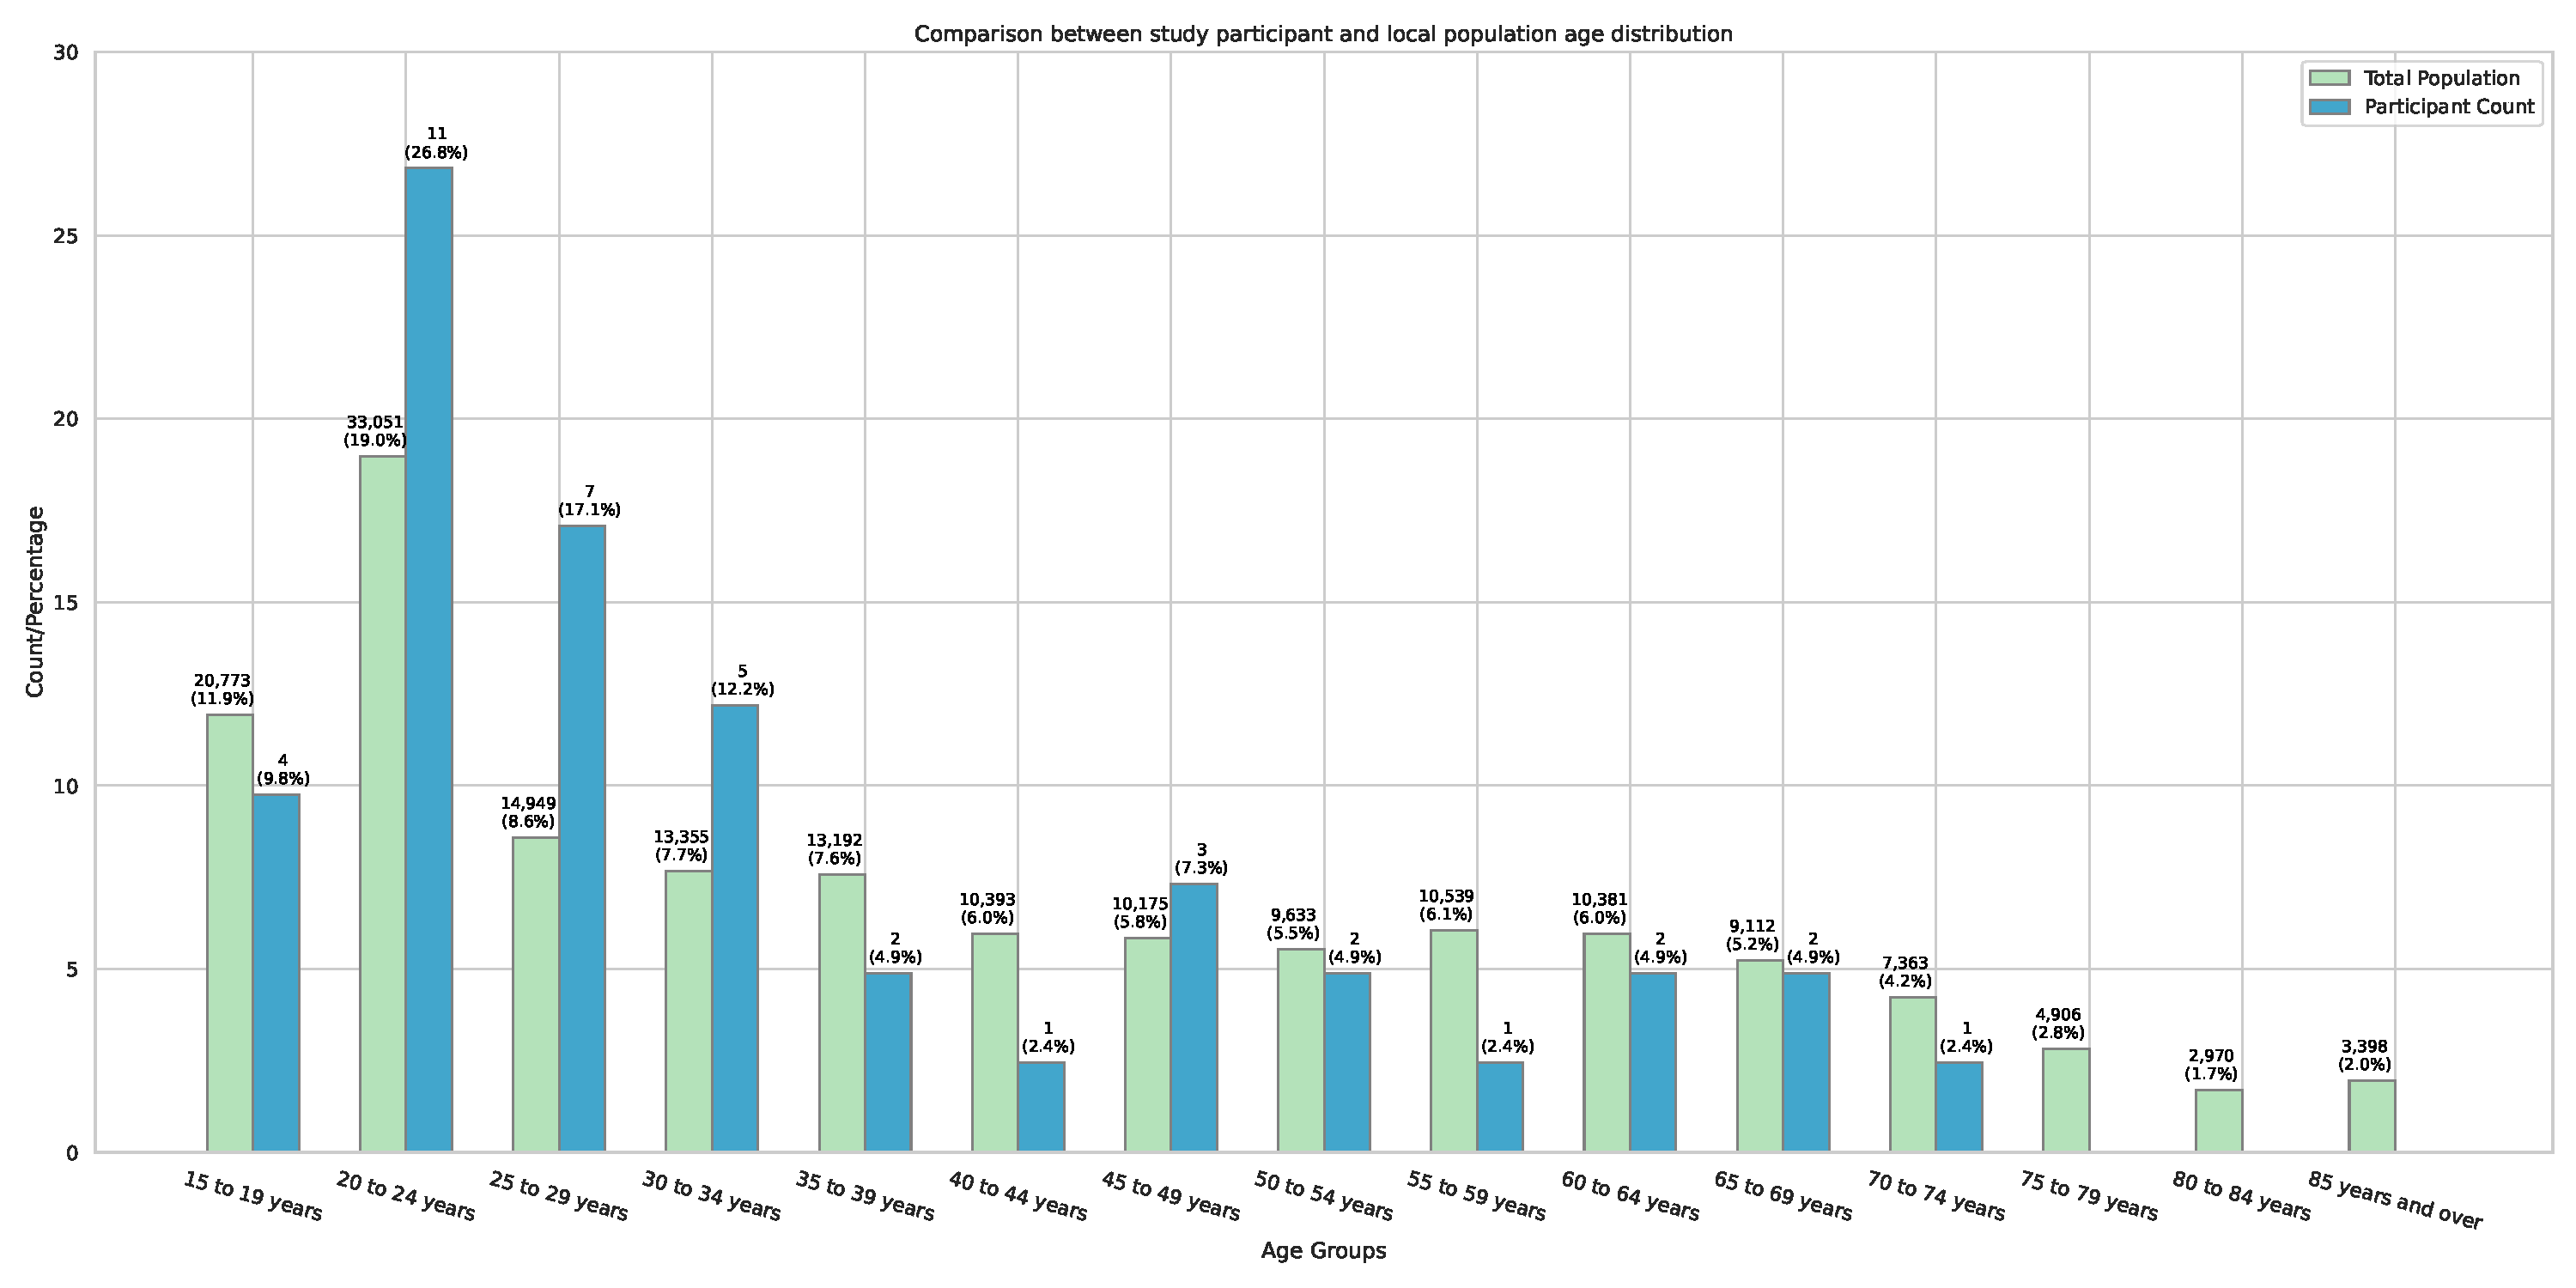
\includegraphics[width=\textwidth]{content/image/demo/demo_age_group_vertical.pdf}
        \caption{Age distribution}
        \label{fig:demoAge}
    \end{subfigure}
    
    \vspace{0.5cm} % Add some vertical space between the rows

    % Bottom figures
    \begin{subfigure}[b]{0.45\textwidth}
        \centering
        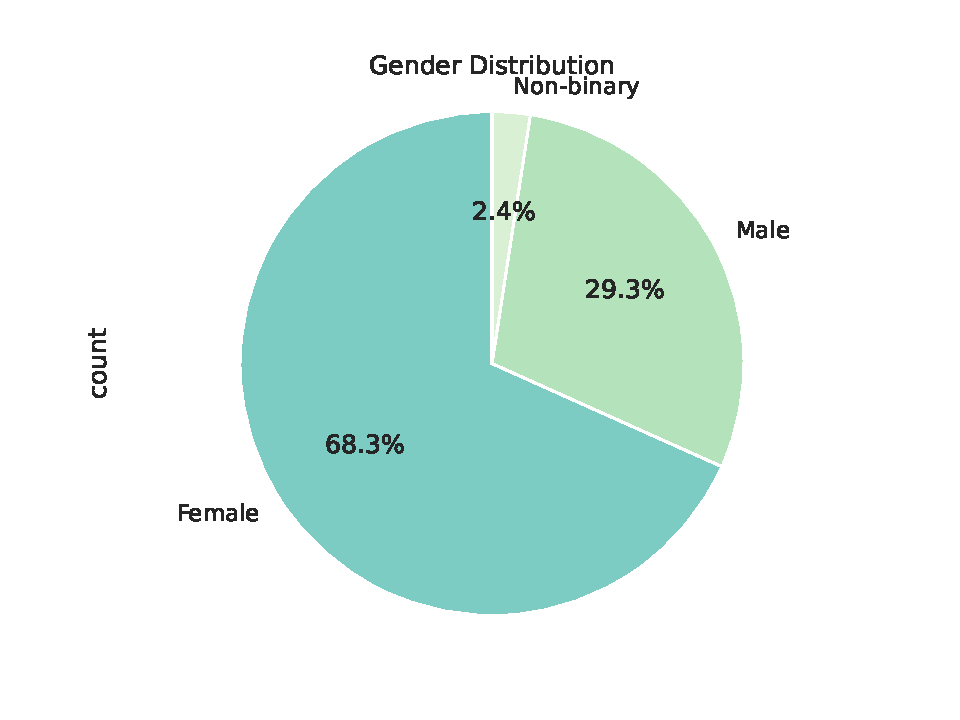
\includegraphics[width=\textwidth]{content/image/demo/demo_gender.pdf}
        \caption{Gender distribution}
        \label{fig:demoGender}
    \end{subfigure}
    \hfill
    \begin{subfigure}[b]{0.45\textwidth}
        \centering
        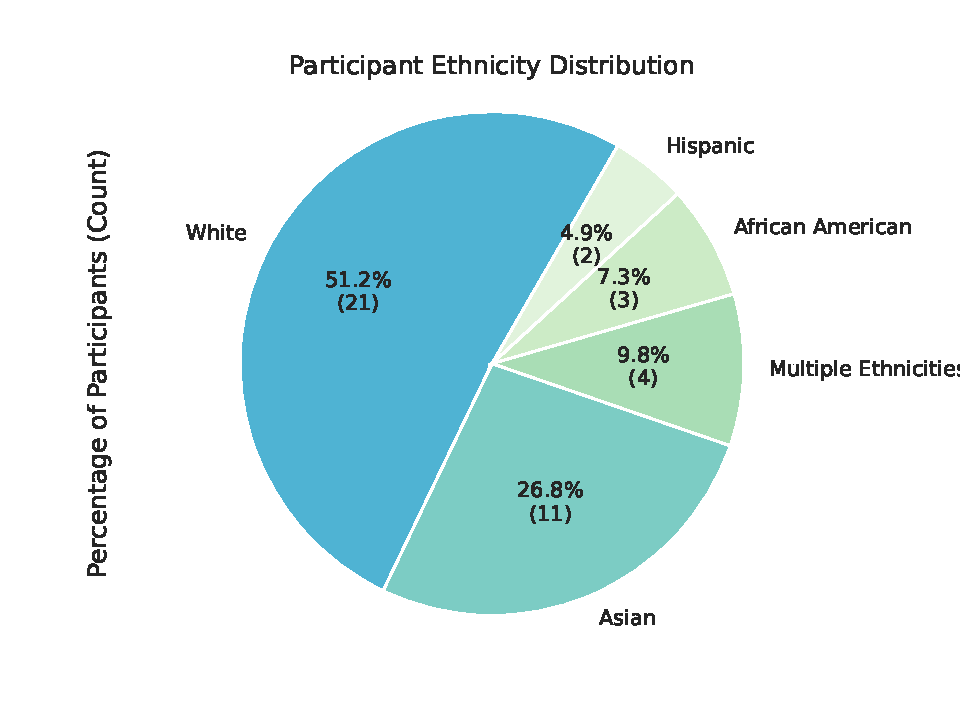
\includegraphics[width=\textwidth]{content/image/demo/demo_ethnicity.pdf}
        \caption{Ethnicity distribution}
        \label{fig:demoEthnicity}
    \end{subfigure}
    
    \caption{Demographic distributions: Age, Gender, and Ethnicity}
    \label{fig:Demographics}
\end{figure}

% maybe more the figure to the appendix?

\vk{the binning here feels a bit narrow for how I feel like age is usually reported. Also is the 15-19 bin not just 18, and 19? Since 15 year olds weren't included, I probably wouldn't compare our percent to the national average}

\section{Cognitive Load across interface and their sources}
\label{sec:cog_result}
In this section, we present the cognitive load across experiment groups, followed by the sources contributing to each cognitive load dimension. Given the limited number of participants, we focus on descriptive quantitative statistics and qualitative assessments of cognitive load. Quantitative data includes metrics collected during the survey tasks, while qualitative insights were generated from post-survey interviews, which were transcribed and thematically analyzed by the first author.

The results are organized as follows: We start with a description of participant demographics, followed by an overview of our cognitive load findings. We then examine six dimensions used in the NASA-TLX survey in the following order: mental demand, physical demand, temporal demand, performance, effort, and frustration. 

\subsection{Demographics}
We recruited a total of $41$ participants, allocating ten to each experiment condition. Due to data quality concerns, we excluded one participant's data\footnote{The participant expressed the experiment as a fake setup that they do not need to complete it seriously.}. The mean age of the participants was $34.63$ years old, with a detailed age distribution presented alongside the county population distribution in Figure~\ref{fig:demoAge}. This comparison reveals that our sample closely matches the county's demographic profile, albeit with a slightly higher representation of younger adults, particularly in the 35-45 age range. As shown in Figure~\ref{fig:demoGender}, the majority of participants skewed toward female.

Regarding ethnicity, $51.2\%$ of the participants identified as White, $26.8\%$ as Asian, $7.3\%$ as African American and $4.9\%$ as Hispanic. Additionally, $9.8\%$ of participants reported mixed ethnicity.

\subsection{Overall Cognitive Load}
\label{sec:cog}
\begin{figure}[ht]
    \centering
    \begin{subfigure}[b]{0.45\textwidth}
        \centering
        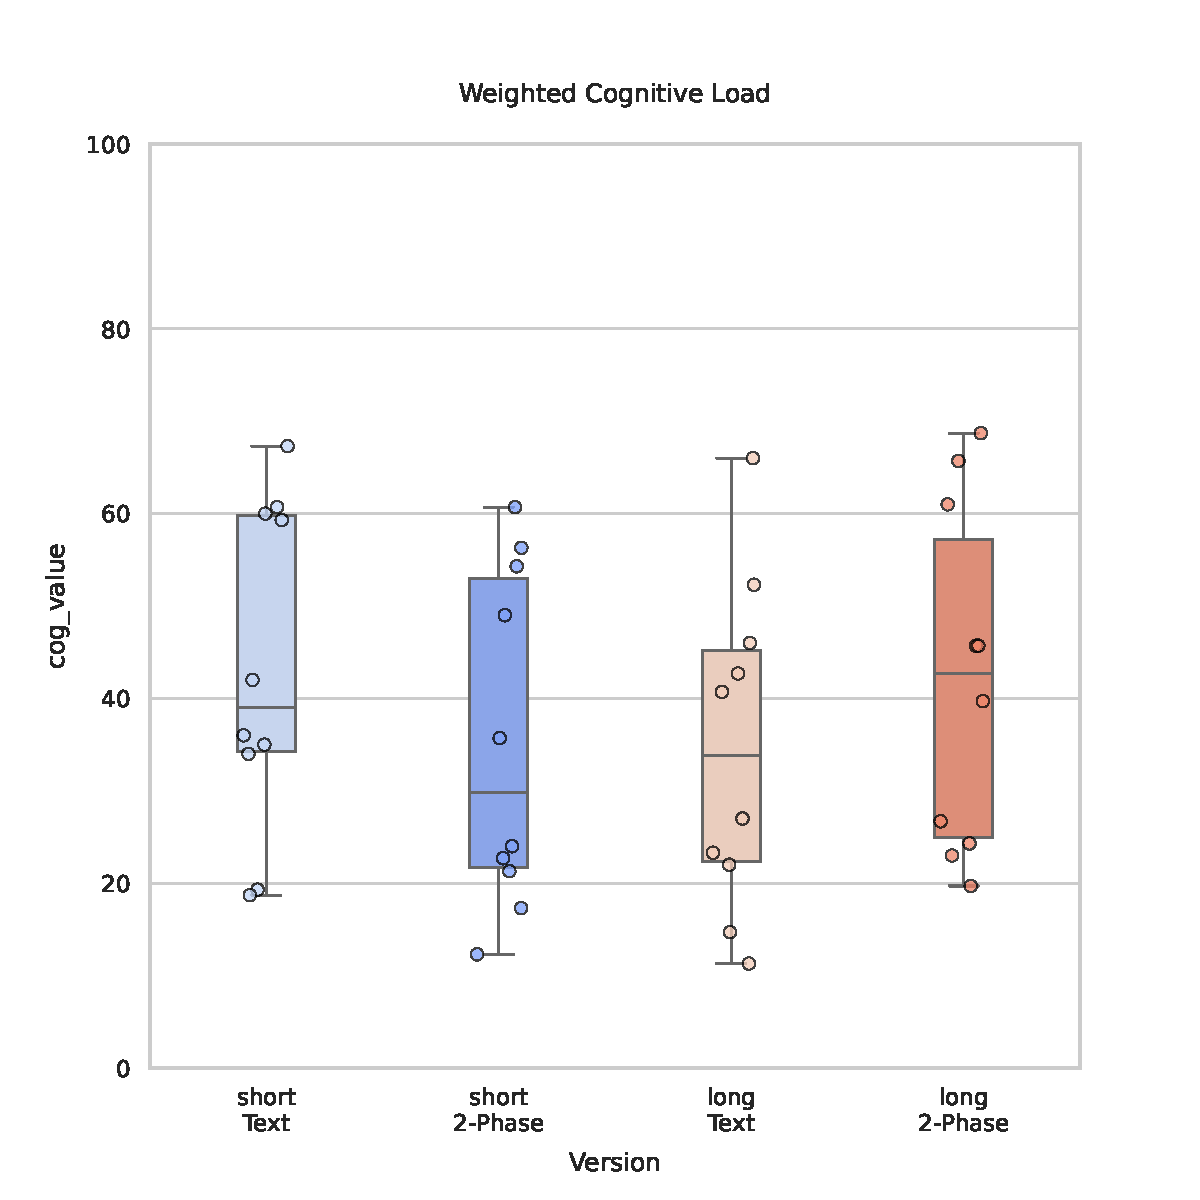
\includegraphics[width=\textwidth]{content/image/results/nasatlx_final_value.pdf}
        \caption{NASA-TLX Weight Score Distribution}
        \label{fig:nasatlx-final1}
    \end{subfigure}
    \hfill
    \begin{subfigure}[b]{0.47\textwidth}
        \centering
        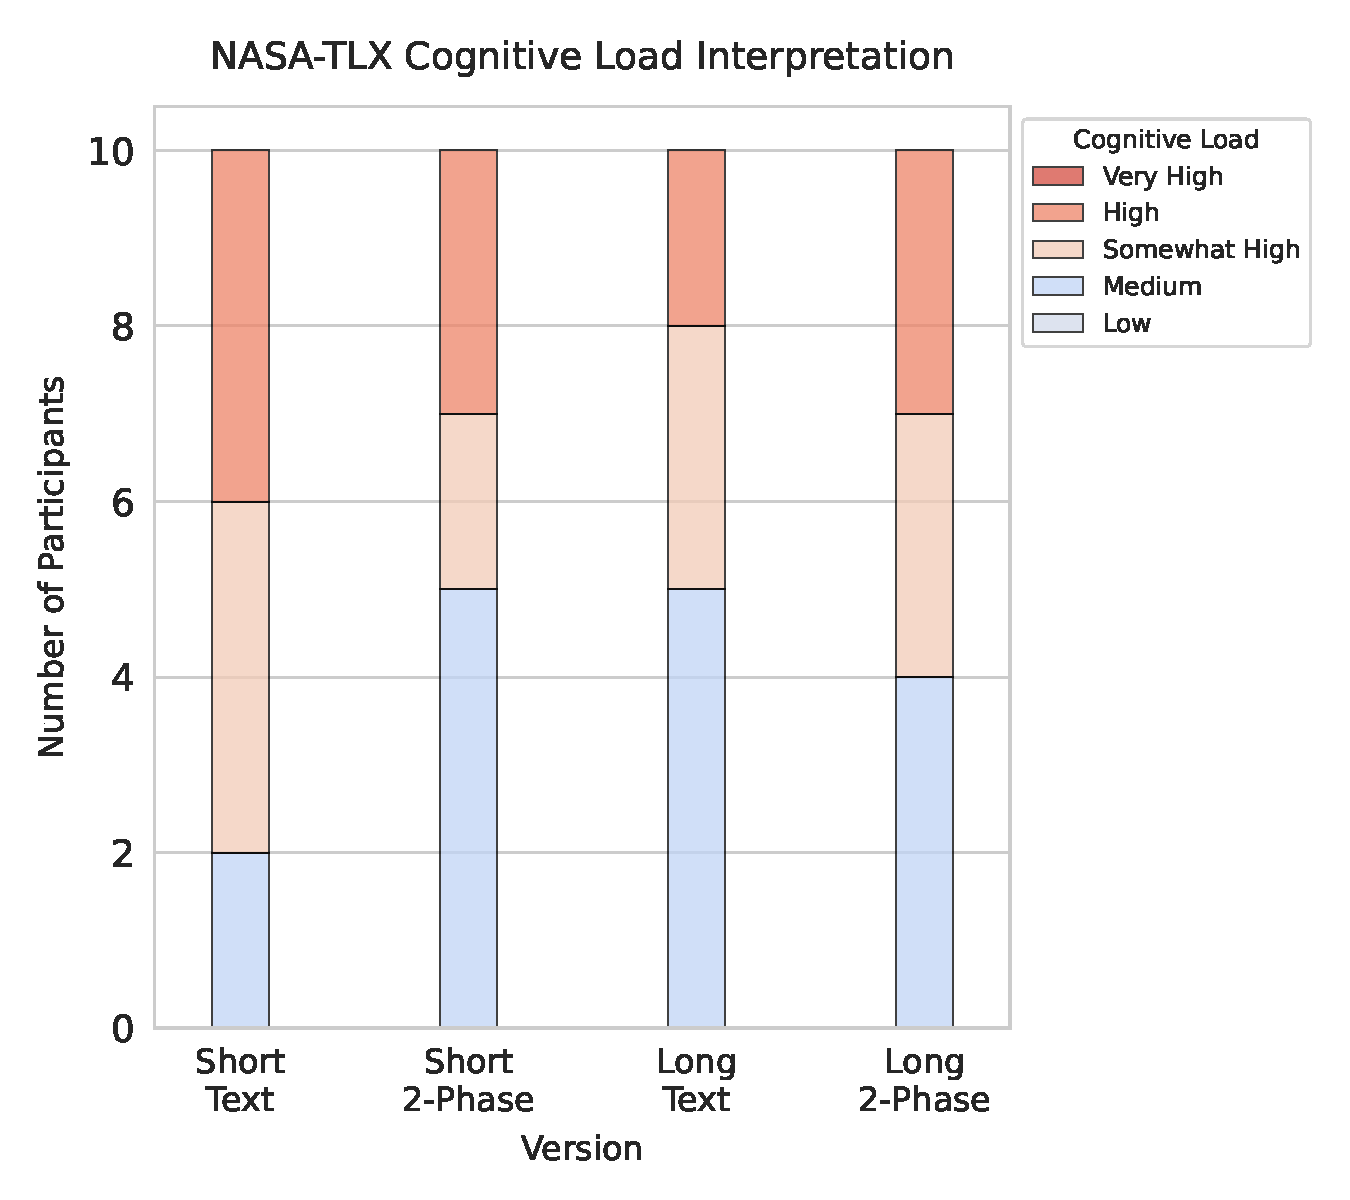
\includegraphics[width=\textwidth]{content/image/results/nasatlx_cog_value_interpreted.pdf}
        \caption{NASA-TLX Cognitive Interpretation}
        \label{fig:nasatlx-final2}
    \end{subfigure}
    \caption{NASA-TLX Results}
    \label{fig:nasatlx-final}
\end{figure}

To answer~\textbf{RQ1} and~\textbf{RQ2a}, we derive the weighted NASA-TLX scores across the four experiment conditions. We show these results in Figure~\ref{fig:nasatlx-final}. Weighted NASA-TLX uses a continuous 0-100 score, with higher values indicating greater cognitive load. We use predefined mappings of NASA-TLX values to cognitive levels: low, medium, somewhat high, high, and very high, as listed by~\textcite{hart1988development}. We show value interpretations in Figure~\ref{fig:nasatlx-final2}. We found that:

\begin{itemize}
    \item Short text interface: The median cognitive load was $39.00$, with a mean of $43.23$ and a standard deviation of $17.65$. $8$ participants reported somewhat high or above, with $4$ reporting high cognitive load.
    \item Short interactive interface: The median cognitive load was $29.85$, with a mean of $35.36$ and a standard deviation of $18.17$. $5$ participants reported somewhat high or above, with $3$ reporting high cognitive load.
    \item Long text interface: The median cognitive load was $33.85$, with a mean of $34.60$ and a standard deviation of $17.69$. $5$ participants reported somewhat high or above, with $2$ reporting high cognitive load.
    \item Long interactive interface: The median cognitive load was $42.70$, with a mean of $42.02$ and a standard deviation of $18.48$. $6$ participants reported somewhat high or above, with $3$ reporting high cognitive load.
\end{itemize}

These results partially answer our first two research questions. First, across the short survey, the interactive interface decreased cognitive load compared to the text interface. This is evident from the median cognitive load decrease from $39.00$ to $29.85$, with more participants reporting lower cognitive load using the interactive interface. The short text interface had the most participants ($N=8$) rating their cognitive load as somewhat high or above. The other three conditions had similar distributions, with about half experiencing medium and half somewhat high or high loads.

Second, contrary to our expectations, the long text interface had a lower cognitive load than the long interactive interface. The cognitive load for the long text interface was even lower than that for the short text interface, with a median cognitive load of $33.85$ compared to $39.00$ in the short text interface. This is counterintuitive, as prior literature suggests that more options can heighten cognitive load~\cite{swellerCognitiveLoadTheory2011}.

By deduction, if the interactive interface increased cognitive load in the long survey, we might expect a similar increase in the short interactive interface compared to the short text interface. However, we observed a lower cognitive load in the short interactive interface. This discrepancy suggests two plausible explanations:

\paragraph{Cognitive Overload Prevention by Interactive Interface} The long survey caused cognitive overload, but the interactive components may have prevented participants from taking mental shortcuts, which would typically reduce measured cognitive load~\cite{daniel2017thinking, simonBehavioralModelRational1955, payneAdaptiveStrategySelection1988, tverskyJudgmentsRepresentativeness}. This prevention could result in a higher cognitive load in the long interactive interface compared to the long text interface. In other words, the interactive interface may have shifted participants' cognitive load from some dimensions to others, maintaining their overall cognitive load at a higher level but not overloaded. If this is true, we expect to see differences among the qualitative explanations of sources, specifically differences in the perceived causes of cognitive load. We will explore this in the next subsections (Subsections~\ref{sec:mental}-\ref{sec:fustration}).

\paragraph{A Pure Increase of Cognitive Load Due to Interactivity} It is also possible that the long survey introduced cognitive overload, and the interactive interface did not influence participants' preference construction but only increased cognitive load due to the added interactivity. In other words, participants are asked to perform additional operations with interactive elements that contributed to a higher cognitive load without providing sufficient cognitive benefits. If this is true, we should expect behavior data to show similar voting patterns across conditions, as the added interactions primarily focused on pre-organization of the options rather than influencing the decision-making process itself. We will explore this in the section~\ref{sec:behave_result}

We also acknowledge the possibility that the elicited values are pure noise and do not reflect the actual cognitive load. This could be due to the small sample size, the nature of the task, or the participants' understanding of the cognitive load scale. While this might be true for small sample sizes, we believe that the qualitative insights from the interviews provide a more nuanced understanding of the cognitive load sources. We detail these limitations in Section~\ref{sec:limitations}.

/hs{ what was your process to identify themes?}
/hs{Section 5.3 (snd section 5 overall) is too long. 

Instead, you could break up section 5 into two sections, one on cognitive  load analysis and the other on behavioral analysis. 

You need to explain in some detail, how you identified the codes for each facet; did you follow a well established process (cite). It'll be nice if you can add a table to summarize the statitucs from the qualitative sections (e.g. how many in each of the experimental consitions felt tha budget management was important to mental demand), You have all the data in the text, and a table would be helpful 

In this new section 5, have a subsection for each of the six facets. Then, take each the six subfigures of fig 12, and use either a wrapfig environment or a side caption figure to insert each of the six subfigures into each of the subsections of this new section 5; this way, the figure will be adjacent to the text for enhanced readability.

Each of the subsections corresponding to each of the dimensions of the scale, you should conclude with a takeaway mesaage. There is so much text here, and it will be easy to be lost.

Section 5.5 and 5,6 should be in the behavioral analysis section

Section 5.7 should be in a discussion section}

% ============================================= %
\begin{table}[h]
    \caption{Mental Demand Table, needs to be updated with some new terms definitions for some of the columns.}
    \label{tbl:mental}
    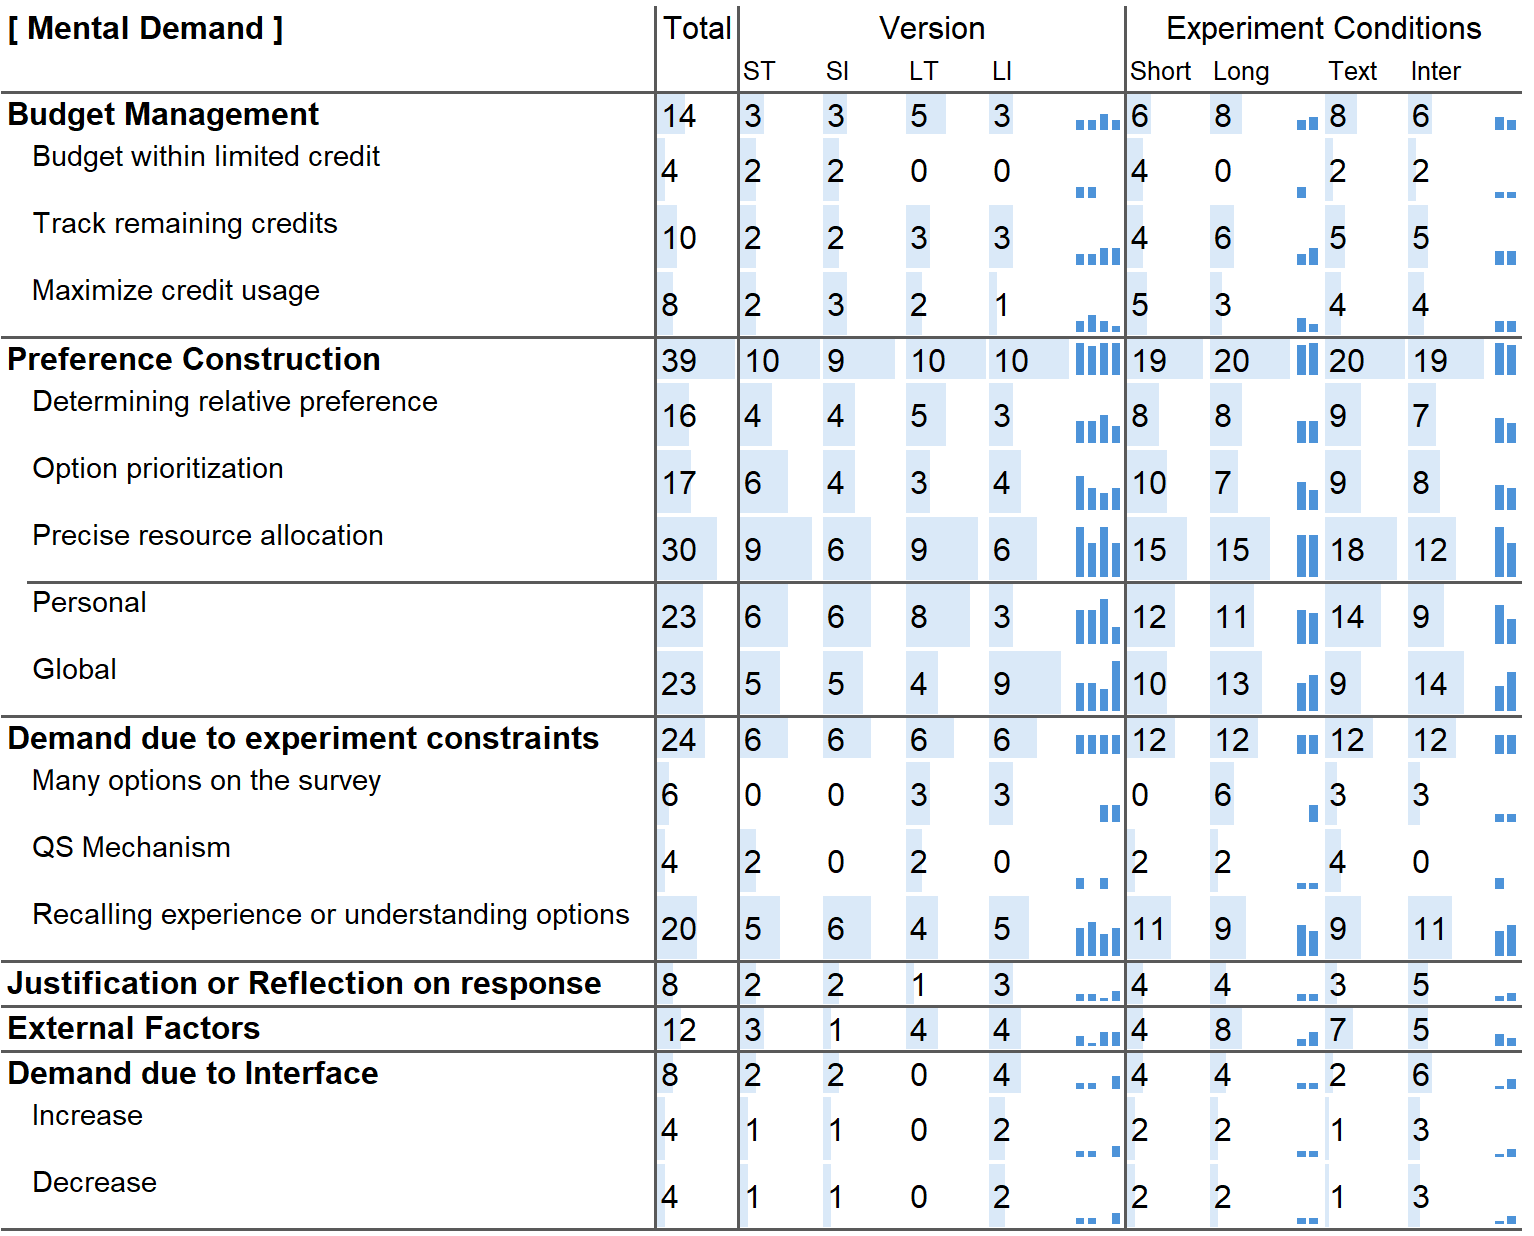
\includegraphics[width=\linewidth]{content/image/cog/mental_table.png}
\end{table}
\subsection{Source of Mental Demand}
\label{sec:mental}

\vspace{5pt}
\begin{tldrbox}
    \faInfoCircle~\xspace\textbf{Takeaway:} Participants across all groups highlighted \textit{Budget management}, \textit{Preference construction}, and \textit{Justification and response reflection} as cause of mental demand. We observed two notable difference: First, slightly more participants using the text interface reported mental demand from precisly determining number of votes for options compared to the interactive interface. Second, when it comes to long QS, participants using the long interactive interface considered broader societal impacts and evaluated options holistically compared to those in the long text interface, who focused on personal relevance and individual issues. 
\end{tldrbox}

Mental demand refers to the extent of mental and perceptual activity required. From the interview results, among all sources contributing to the increase of mental demand, we identified two major sources contributing to mental demand:~\textit{Budget management} and~\textit{Preference construction}. A detailed breakdown of participant distribution across different sources that influenced their mental demand is presented in Table~\ref{tbl:mental}. While $24$ participants mentioned experiment setup, most of them attributes it to understanding and recalling their experience related to the option. The other three sources directly associated with completing QS include: \textit{Budget management}, \textit{Preference construction}, and \textit{Justification and response reflection}.

\subsubsection{Mental Demand Source: Budget management} $14$ participants expressed demand from trying to budget within limited credit ($N=4$), track remaining credits ($N=10$), and maximize the use of credits ($N=8$). For example:

\begin{displayquote}
How many I got left that~\ldots\ that I haven't voted on yet, and seeing if I and looking at the remaining credits, I'm trying to mentally divide that up before I start allocating upvotes and downvotes.

\small{\noindent \hfill -- S006, long interactive interface, budget within limited credit}
\end{displayquote}

\begin{displayquote}
And then I just wanted to make sure that I used all the credit that I had available to me, and also knowing that in order to like show your support for certain societal issues you had to like that was giving a tangential take away from other societal issues that you could support as well.
    
\noindent \hfill -- S032, short text interface, track remaining credits.
\end{displayquote}

In the first quote, the participant struggles with not running out of credit while allocating credits to options they haven't yet attributed. The second quote highlights the challenge of maximizing spend while ensuring sufficient differentiation. All these factors relate to effective budget management.

\subsubsection{Mental Demand Source: Preference construction} Almost all participants ($N=39$) experienced an increase in mental demand due to preference construction. This can be broken down into three sources: determining relative preference ($N=16$), where participants focus on internal evaluation and comparison among different options; option prioritization ($N=17$),  where participants make trade-offs to identify high-priority options and translate internal preferences into a subset of options; and precise resource allocation ($N=30$), where participants allocate specific values or adjustments to represent their preferences. For each of these sources, we show an example:

\begin{displayquote}
Figuring out my priorities, and how much I prioritize option 1 over option 2. What is the difference between those 2 on my priority list?

\hfill -- S002, short interactive interface, determining relative preference
\end{displayquote}

% I think the whole time I was trying to balance, I think II think I partly was discovering my what's the word I want to use bias isn't quite right. My priorities (S031, I)

\begin{displayquote}
I knew which ones that I wanted to dedicate the most to, and I knew which one I wanted to dedicate the least to. But it was that middle area that was kind of a grey area.
    
\noindent \hfill -- S008, short interactive interface, option prioritization
\end{displayquote}

% I knew which ones that I wanted to dedicate the most to, and I knew which one I wanted to dedicate the least to. But it was that middle area that was kind of a grey area.
% \noindent \hfill -- S024, short text interface, option prioritization

\begin{displayquote}
I'm not sure how to put into words~\ldots like having to pick how many upvotes would go to each one
    
\noindent \hfill -- S023, long text interface, precice resource allocation
\end{displayquote}

Almost all participants mentioned preference construction as a source of mental demand, echoing the theory that preference construction is a difficult and mentally demanding task. In addition, we notice slightly more participants using the text interface cited the cause of mental demand from precise resource allocation compared to the interactive interface ($18$ verses $12$). We conjecture that participants, with the help of the interactive interface, might have been able to make more informed decisions and thus experienced less mental demand in this area.

\subsubsection{Mental Demand Source: Justification and response reflection} $8$ participants expressed mental demand from justifying their choices and reflecting on their responses ($N=4$). Participants would either reflect whether the votes they allocated reflected their true preferences or whether the among of credit spent is worth it.

\begin{wrapfigure}{r}{0.45\textwidth} % Adjust the width as needed
    \centering
    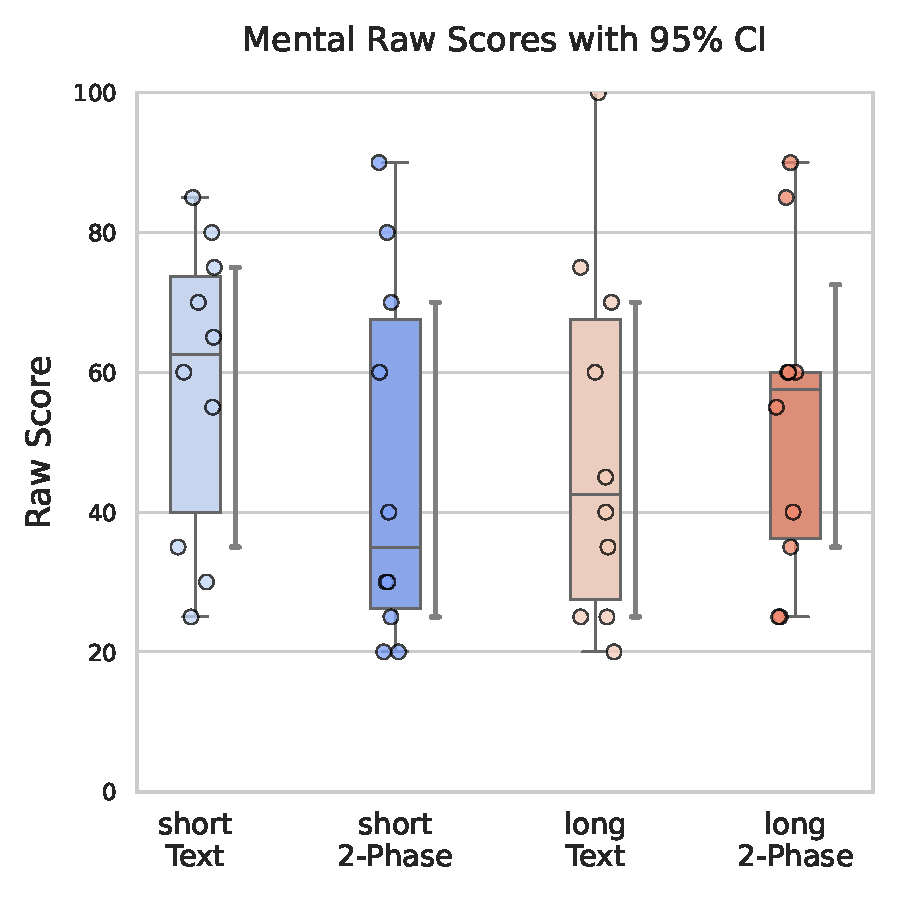
\includegraphics[width=0.45\textwidth, trim=0 13 0 13, clip]{content/image/cog/Mental_scores.pdf}
    \captionsetup{width=0.40\textwidth, justification=justified} % Adjust the width to match the image width
    \caption{Mental Demand Raw Score: Across all four experiment groups, participant's reported mental demand is spread across a wide range with many participants experiencing high mental demand.}
    \label{fig:mental_cog_score}
\end{wrapfigure}

\subsubsection{Long QS Conditions: A different scope of preference construction and budget management approach}

While these sources are common across all experiment groups, we highlight a notable difference when we focus on participants across interfaces completing the long QS.~\textbf{They focus on a different scope of preference construction}.More specifically, participants ($N=8$) in the long text interface tend to experience mental demand from preference construction by thinking about issues more narrowly and focusing on personal relevance. Conversely, participants ($N=9$) in the long interactive interface experience higher mental demand from considering the broader societal impact and evaluating options more holistically. Only four participants in the long text interface expressed a holistic view, and three participants in the long interactive interface expressed a narrow and personal view.

/hs{What is "a holistic view"? why is it about the long text interface that prevents them evaluating options holistically?}
/tc{Conjecture: choice overload -> heuristics -> so they become narrower}
% \begin{displayquote}
% \bracketellipsis also seeing the long list and obviously having to pick between quite a few things that I do feel very strongly about and having to figure out which ones do, I feel more strongly about than others.
    
% \noindent \hfill -- S023, long text interface
% \end{displayquote}

\begin{displayquote}
Trying to figure out what upvotes I should give it you know~\ldots compared to~\ldots I even kind of went back compared to the other topics: <topic one> compared to <topic two>, and even with like <topic three>, I kind of went back and forth between those two. \bracketellipsis So it was very mental tasking for me.

\noindent \hfill -- S015, long text interface
\end{displayquote}

% \begin{displayquote}
% \bracketellipsis really having to think, especially with so many different societal issues. How do I personally prioritize them? And to what extent do I prioritize them?
    
% \noindent \hfill -- S009, long interactive interface
% \end{displayquote}

\begin{displayquote}
\bracketellipsis really going through the rest of the categories and deciding okay, which are the pressing issues of our time and which are the pressing issues for this particular society that that I live in. \bracketellipsis You know these causes need a lot more funding, and and others can probably still have some sort of an impact, even with less resources.

\noindent \hfill -- S019, long interactive interface
\end{displayquote}

In the first quote, participants expressed mental demand narrowly focused on three options, trying to recall specific characteristics to differentiate among the options. In the second quote, participants consider how options play a role in society and the bigger picture, aiming to maximize impact. This difference indicates a shift in cognitive load from personal relevance to societal impact across the two long QS conditions. We conjecture that this represents participants in the long text interface are applying heuristics to narrow down their choices, while participants in the long interactive interface are considering a broader range of factors to make their decisions through the scaffolding provided by the interactive interface. 

/hs{put everything related to budget in one place; right now, you have budget, -> pref -> budget }/tc{TODO: Need to get the values of the participant count.}
In addition, we also find that long text interface participants focused on more operational behaviors such as:

\begin{displayquote}
So I wanted to be fair.~\bracketellipsis I actually took my calculator out and said~\bracketellipsis  how much would it be if I equally distributed it and then how do I do that? Do I wanna do it all equally or not?

\noindent \hfill -- S020, long text interface
\end{displayquote}

compared to more procedures involving more strategic planning such as:

\begin{displayquote}
I wanted to make sure I wanted to give some credit to everything~\bracketellipsis I'm trying to make sure that I had without doing a lot of~\ldots I guess redos is trying to kind of get it right the first time on how I weight things.

\noindent \hfill -- S032, long interactive interface
\end{displayquote}

Strategic planning does not refer to gaming out others or 'winning' a game but rather to high-level thinking processes that consider strategies and plans to tackle a challenge, compared to operational tasks such as adjusting a specific vote value. While we did not notice significant differences in mental demand raw values (Figure~\ref{fig:mental_cog_score}) across the four experiment groups, the different actions regarding budget management and preference construction show a shift in mental demand across experiment conditions.

% IN_T4: Wanting more information on the options (N=6/40)
% 5. While the numbers seem small, non of this request came from v3. This could explain that participants are already overloaded from the existing the task.

% ============================================= %
\begin{table}[h]
    \caption{Mental Demand Table, needs to be updated with some new terms definitions for some of the columns.}
    \label{tbl:physical}
    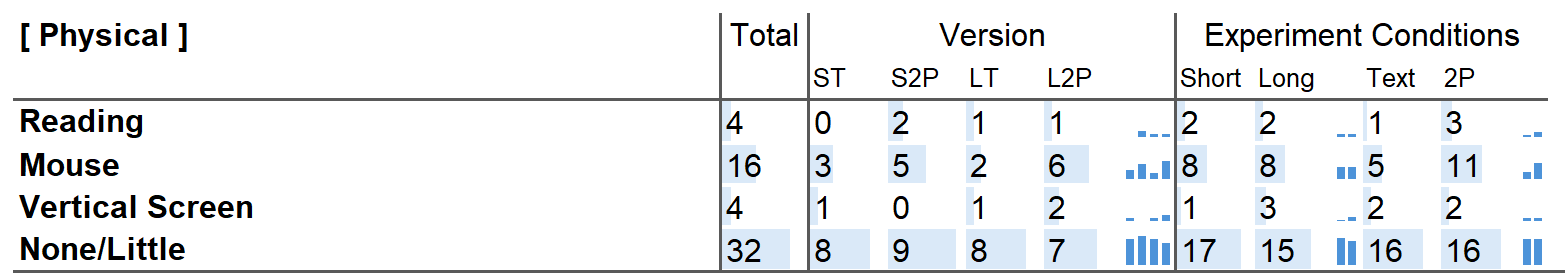
\includegraphics[width=\linewidth]{content/image/cog/physical_table.png}
\end{table}
\subsection{Source of Physical Demand} 
\label{sec:physical}

\vspace{5pt}
\begin{tldrbox}
    \faInfoCircle~\xspace\textbf{Takeaway:} Participants across all groups highlighted \textit{Reading}, \textit{Using the mouse}, and \textit{navigating a vertical screen} as cause of physical demand. Most participants experienced little or minimal physical demand. Table~\ref{tbl:physical} shows the distribution of participants across different sources of physical demand.
\end{tldrbox}

\begin{wrapfigure}{r}{0.45\textwidth} % Adjust the width as needed
    \centering
    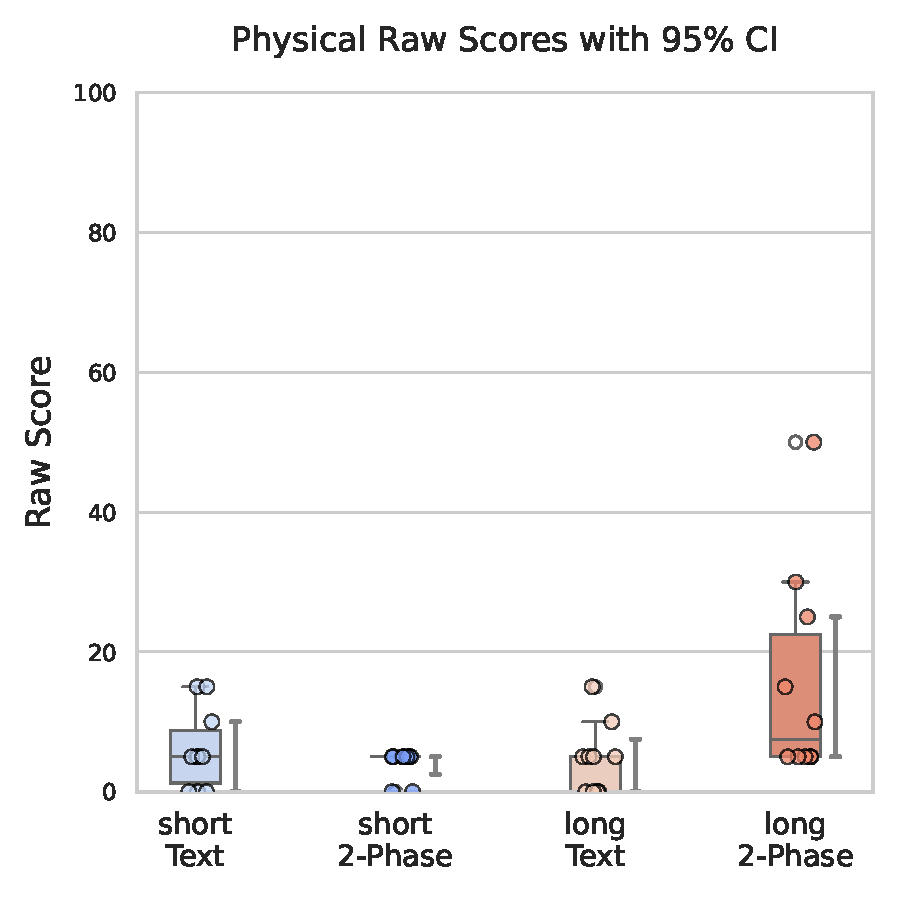
\includegraphics[width=0.45\textwidth, trim=0 13 0 13, clip]{content/image/cog/Physical_scores.pdf}
    \captionsetup{width=0.40\textwidth, justification=justified} % Adjust the width to match the image width
    \caption{Physical Demand Raw Score: Participants other than the long interactive interface reported minimal physical demand. The long interactive interface had the highest physical demand, likely due to increased mouse clicks and extended time spent looking at the vertical screen.}
    \label{fig:physical_cog_score}
\end{wrapfigure}

Physical demand refers to the physical effort required to complete a task, such as physical exertion or movement. Since this study involves participants sitting in front of a computer screen completing a survey, most participants reported minimal physical demand($N=32$). We nonetheless report the sources of this minimal demand, which include reading text on the screen ($N=4$), using the mouse ($N=16$), and moving their head to navigate the vertical screen ($N=5$). Participants emphasized that these demands were minimal, which is reflected in the low values reported in the NASA-TLX physical demand scores (Figure~\ref{fig:physical_cog_score})

Notably, $11$ out of $20$ participants that used the interactive interface mentioned physical demand from using the mouse, reflecting their increased interaction with the interface. This is further supported by the raw NASA-TLX physical demand scores, which show a significance difference visually between short and long interactive interfaces as well as between text and interactive interfaces in long surveys. \hs{Would it be possible to not use NHST? It's difficult to convince a reviewer that you have statistical significance with a small subject pool ; the study is underpowered}

% ============================================= %
\newpage % TODO: this is a temp solution, need to fix toward the end
\begin{table}[h]
    \caption{Temporal Demand Table, needs to be updated with some new terms definitions for some of the columns.}
    \label{tbl:temporal}
    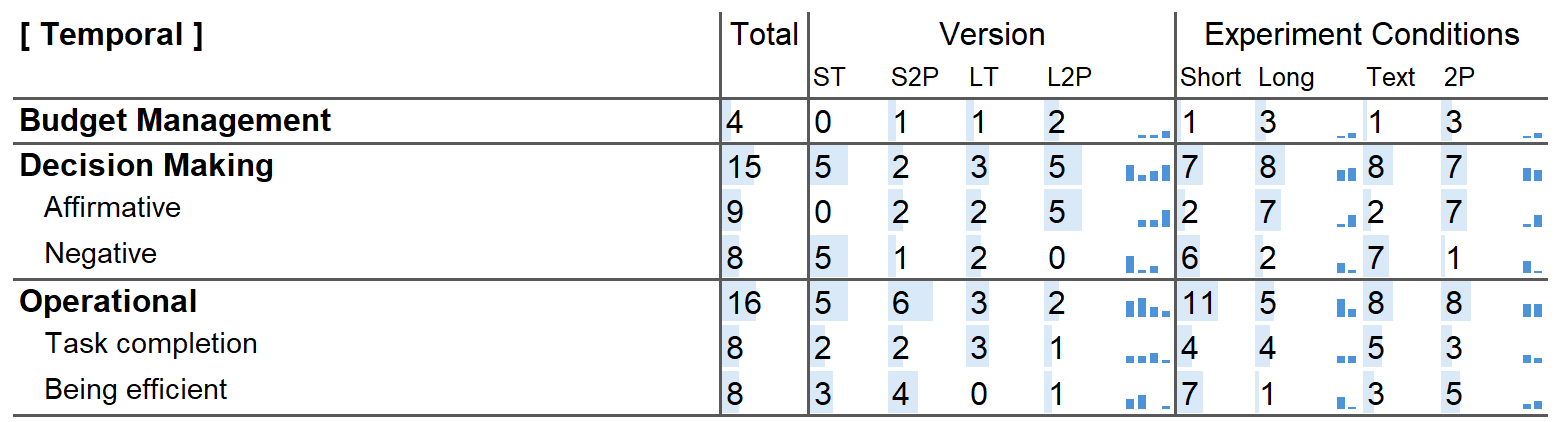
\includegraphics[width=\linewidth]{content/image/cog/temporal_table.png}
\end{table}

[I am some text before I can fix the layout.]

\subsection{Source of Temporal Demand} 
\label{sec:temporal}
\vspace{5pt}

\begin{tldrbox}
    \faInfoCircle~\xspace\textbf{Takeaway:} Participants experienced increased temporal demand due to three main sources: \textit{Budget}, \textit{Decision Complexity}, and \textit{Operational Efficiency}. Notably, participants in the short text interface were highly sensitive to sunk cost effects, leading to a higher temporal demand. Table~\ref{tbl:temporal} shows the distribution of participants across different sources of temporal demand.
\end{tldrbox}

Temporal demand refers to the time pressure felt by the participant while performing a task. A lower temporal demand suggests participants experience a slow and leisurely pace. The themes we uncovered from the interviews consist of three main sources that lead to participants' increase in temporal demand. These include:~\textit{Budget}, ~\textit{Decision Complexity}, and ~\textit{Operational Efficiency}. 

\subsubsection{Budget}
Budget is a lightly discussed theme that emerged across experiment conditions. Four participants mentioned budget increasing their temporal demand. Although budget can only decrease through spending, it is interesting that some participants expressed that the reduction in credit value created a sense of time pressure. Participants translated the increasing marginal cost of votes into higher temporal demand. As one participant said,

\begin{displayquote}
When the money was decreasing, as I was casting more upvotes or downvotes so as the money decreases I felt kind of rushed.
            
\noindent \hfill -- S034, long interactive interface
\end{displayquote}

\subsubsection{Decision Complexity} Decision Complexity refers to when participants felt that there are many decisions to make. These causes are expressed in two forms—affirmative and negative. Affirmative perception refers to participants explicitly expressing that there are many decisions to make, while negative perception refers to participants describing concerns regarding the time and effort already invested in the survey.

\begin{displayquote}
So it didn't take too much time but obviously there was a lot of things to consider. So there was some temporal demand.
    
\noindent \hfill -- S022, short interactive interface
\end{displayquote}

\begin{displayquote}
\bracketellipsis so at first it was like, `Okay, this is fine.' But then on the end, I was like, maybe I should just hurry up and make a decision. So it's like at first it would been here, but then I kinda moved up near the end when I was hanging a waffling between my upvotes.
\noindent \hfill -- S024, short text interface
\end{displayquote}

The former quote pointed out participants making many decisions, while the latter highlighted the increase in temporal demand due to an expected devoted time. What we found important was that each experiment group had participants expressing both perspectives on decision complexity as a source of temporal demand. However, half of the participants ($N=5$) in the short text interface and half of the participants ($N=5$) in long interactive interface expressed concerns due to decision complexity. The long interactive interface involved all five participants registering an affirmative perspective. This is not surprising because participants in the long interactive interface had the most actions needed for organizing and voting. On the other hand, it is interesting to observe that four of these five participants in the short text interface expressed a negative perspective. This indicates that participants in this group are highly sensitive to their sunk cost effect.
% v2 -- 2 and v3 -- 3

\subsubsection{Operational Efficiency}
Unlike decision complexity, which refers to the abundance of decisions to be made, operational efficiency refers to specific and concrete operations or goals. For example, completing the survey, executing an operation, or accomplishing a specific task like updating vote values.

\begin{displayquote}
I wanna get through things in an efficient manner which doesn't necessarily mean I rush it. But it does mean that I do things expeditiously. Especially. I'd like to think I'm somewhat computer-savvy. And so to be able to move through this quickly and efficiently. I do take pride in, but it's all personal stuff. It's not nothing outwardly influencing me. 
        
\noindent \hfill -- S032, short text interface
\end{displayquote}

\begin{displayquote}
I want the credit done but I don't want to be overthinking.
            
\noindent \hfill -- S013, short text interface
\end{displayquote}

The former quote refers to the participant aims to operate swiftly on the interface, not specifically related to decision making. Similarly, the latter focuses on using the credit to complete a specific goal. When asked about temporal demand, 11 participants (five from interactive and six from text interface) out of 20 who responded to the short survey expressed operational efficiency resulting in temporal demand, compared to just five (three from text and two from interactive interface) out of 20 in the long interface group.

\begin{wrapfigure}{r}{0.45\textwidth} % Adjust the width as needed
    \centering
    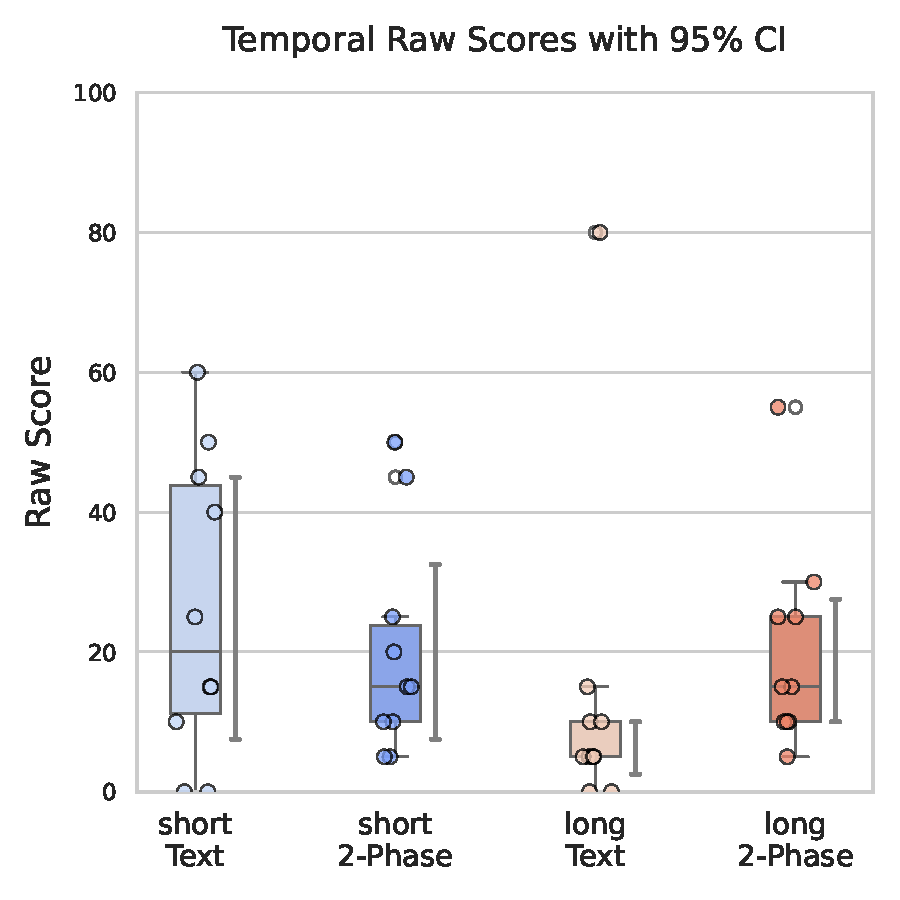
\includegraphics[width=0.45\textwidth, trim=0 13 0 13, clip]{content/image/cog/Temporal_scores.pdf}
    \captionsetup{width=0.40\textwidth, justification=justified} % Adjust the width to match the image width
    \caption{Temporal Demand Raw Score: I am some text that needs to be filled.}
    \label{fig:temporal_cog_score}
\end{wrapfigure}

Taking~\textit{Decision Complexity} and~\textit{Operational Efficiency} altogether, we interpret that the participants in the short survey misperceived the task as simple, seeing just six options on the screen, and thus anticipated the task to be simple and easily completed. We observe similar patterns from the NASA-TLX temporal demand raw values (Figure~\ref{fig:temporal_cog_score}). The short text interface shows a relatively higher demand across the four groups, reflecting the demand from both decision complexity and operational efficiency. This is followed by the short interactive interface, affected by operational efficiency, and the long interactive interface, affected by decision complexity. The long text interface showed the least amount of temporal demand. Our statistical tests showed a significant difference between the long text interface and the long interactive interface ($p<0.05$) after a Mann-Whitney U test.\hs{what is the response variable?}

It is also worth noting that three participants from the 20 who responded to the long survey mentioned that the vertical screen's ability to see all options facilitated direct comparisons and transparency about the entirety of the task, which reduced the temporal demand.

\begin{displayquote}
(Seeing) all at once I can see how many there are, so it's kind of like I can kind of tell when I will be done.

\noindent \hfill -- S041, long text interface
\end{displayquote}

% ============================================= %
\begin{table}[h]
    \caption{Mental Demand Table, needs to be updated with some new terms definitions for some of the columns.}
    \label{tbl:physical}
    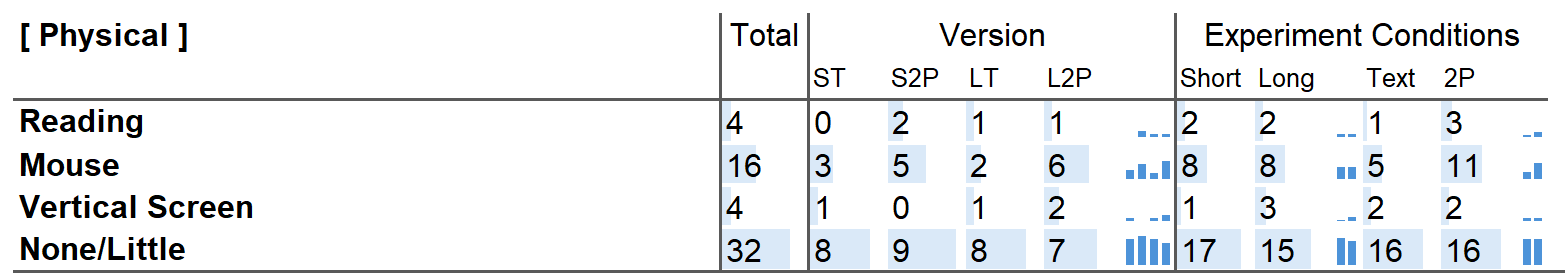
\includegraphics[width=\linewidth]{content/image/cog/physical_table.png}
\end{table}

\subsection{Source of Performance}
\label{sec:performance}
\vspace{5pt}
\begin{tldrbox}
    \faInfoCircle~\xspace\textbf{Takeaway:} Participants experienced performance demand from two main sources: \textit{Operational Actions} and \textit{Social Responsibility}. Operational actions included pressures to use all credits or ensure choices reflected true preferences. Social responsibility included concerns about fairness and the potential impact of decisions. Despite these pressures, participants generally felt positive about their performance, with notable differences in the nature of their satisfaction. Those using interactive interfaces were more likely to express feeling good about their performance, while those using text interfaces were more likely to report they did their best.
\end{tldrbox}

Performance refers to how the person perceived if they successfully completed the task. A lower value refers to a good performance and vice versa. We find less differences between experiment groups qualitatively and quantitatively. However, there are notable takeaways that we can derive from the data.

First, we identified two sources of performance demand:~\textit{Operational Actions} and~\textit{Social Responsibility} from the interviews. 

\subsubsection{Operational Actions}
Similar to previous demands, operational actions refer to specific and executable procedures participants can perform in the survey. These sources are shared across experiment groups. Six participants reported feeling pressured to spend all their credits or ensure they stayed within budget. Five participants were concerned that their choices did not accurately reflect their true preferences. Additionally, six participants mentioned experiencing performance demand due to the limited time, energy, and resources available, which ties into other cognitive demands. Here we show two examples:

\begin{displayquote}
I don't think I did it perfectly, because I didn't have 0 remaining credits.
    
\noindent \hfill -- S024, short text interface, budget management
\end{displayquote}

\begin{displayquote}
I'm concerned that it's not as reflective of my views as I wanted to be like, or I was concerned about it.~\bracketellipsis I was concerned that maybe it didn't.

\noindent \hfill -- S041, long text interface, preference reflectiveness
\end{displayquote}

\subsubsection{Social Responsibility}
Social Responsibility is a noteworthy source of perforamce demand, categorized into accounting~\textit{decision-maker responsibility} (N=8) and from considering~\textit{uncertainity of the outcome} (N=3). The former refers to individuals feeling guilty because they weren't able to avoid because of specific tradeoffs or that they want to be fair. For example, 

\begin{displayquote}
I don't want people to think that I just like don't care about <ethnicity> people at all. I also don't think like government funding should go towards like religious organizations. You know what I mean. So I don't want somebody to think that like, I just don't care about <ethnicity> people.
    
\noindent \hfill -- S041, long text interface, decision-maker responsibility
\end{displayquote}

In this quote, the participant placed themselves inside the shoes of a member of the government, rather than a citizen expressing their own attitudes. This shift in roles introduced the perforamce demand, however, it demonstrated that QS shared decision maker's dilemma to individual survey respondents. This characteristic extends to the latter which further to the participants trying to forsee an outcome:

\begin{displayquote}
If I was actually running a government funding~\bracketellipsis I don't know how this (the survey results) might actually affect people. Some of these things might be unpopular or bad, or have outcomes that I didn't forsee.
    
\noindent \hfill -- S027, short interactive interface, uncertainity of the outcome
\end{displayquote}

\begin{wrapfigure}{r}{0.45\textwidth} % Adjust the width as needed
    \centering
    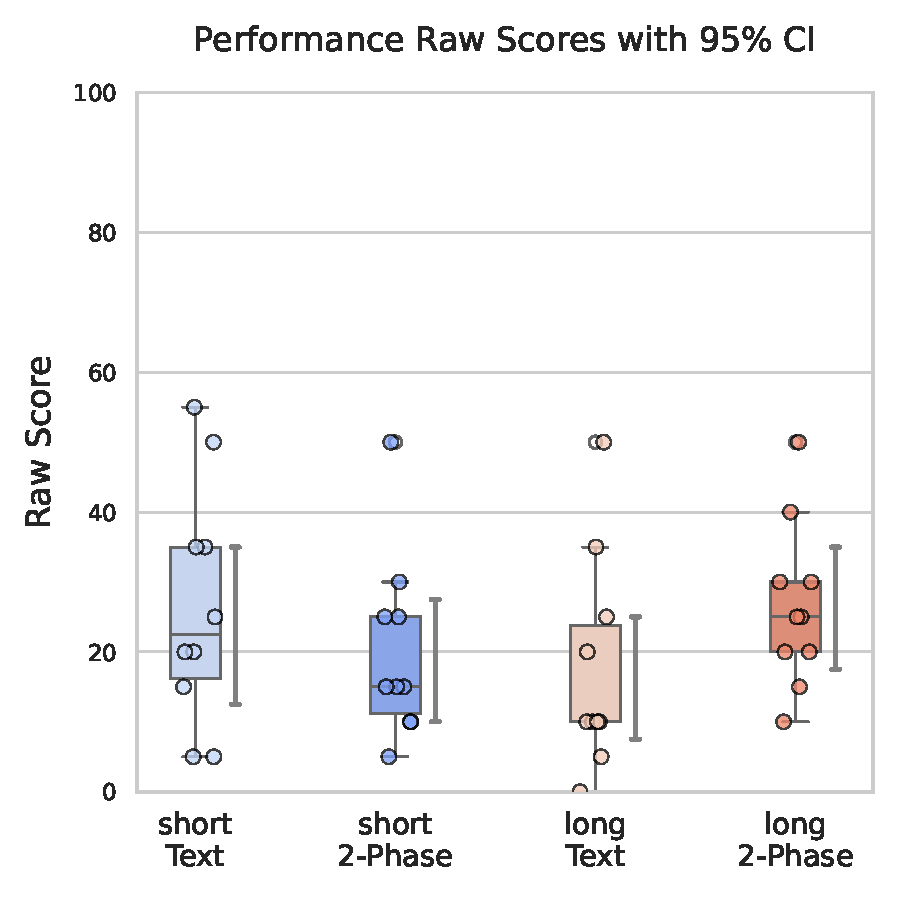
\includegraphics[width=0.45\textwidth, trim=0 13 0 13, clip]{content/image/cog/Performance_scores.pdf}
    \captionsetup{width=0.40\textwidth, justification=justified} % Adjust the width to match the image width
    \caption{Performance Demand Raw Score: Text are placd here.}
    \label{fig:performance_cog_score}
\end{wrapfigure}

Similar to the previous source, social responsibility is also shared across experiment groups. Considering the raw NASA-TLX scores(Figure~\ref{fig:performance_cog_score}), participants expressed similar levels of perforamce score. This aligns with the interview results where most participants felt positive about their final submission. This result is expected because the task is designed to reflect their preferences, not to measure performance. We further analyzed the types of satisfactory statements regarding performance.

\subsubsection{Evaluation of their performance}
We identified three types of satisfactory statements regarding self reported performance:
\begin{itemize}
    \item \textit{Did their best} refers to statements where a participant stated they exhausted their maximum effort to complete the task.
    \item \textit{Feel good} efers to statements where a participant who expressed positive emotions or satisfaction about their performance or the outcome.
    \item \textit{Good enough} refers to statements where a participant acknowledged that their performance or the outcome was acceptable or satisfactory, but not necessarily perfect or the best possible.
\end{itemize}

We found approximately the same number of participants in each of the four experiment groups expressed \textit{Good enough}. Meanwhile, participants using the interactive interface across short and long groups had almost double the number of participants ($N=11$) who expressed \textit{Feel good} compared to the text interface ($N=6$). On the other hand, the text interface had slightly more participants ($N=5$) who expressed \textit{Did their best} compared to the interactive interface ($N=3$).

This result highlights a few important takeaways. First, participants from all experiment groups expressed satisficing behaviors (\textit{Good enough}) with no particular group reporting a higher frequency of this behavior. Second, participants using the text interface are experiencing challenges that make them feel they have to do their best to complete the task. Last, participants using the interactive interface are generally positive about their experience and the outcome.

% TODO: Need to check the reflective thinking part a bit. I **think** there are differences but it is unclear, need to go back to raw code.


% ============================================= %
\begin{table}[h]
    \caption{Mental Demand Table, needs to be updated with some new terms definitions for some of the columns.}
    \label{tbl:physical}
    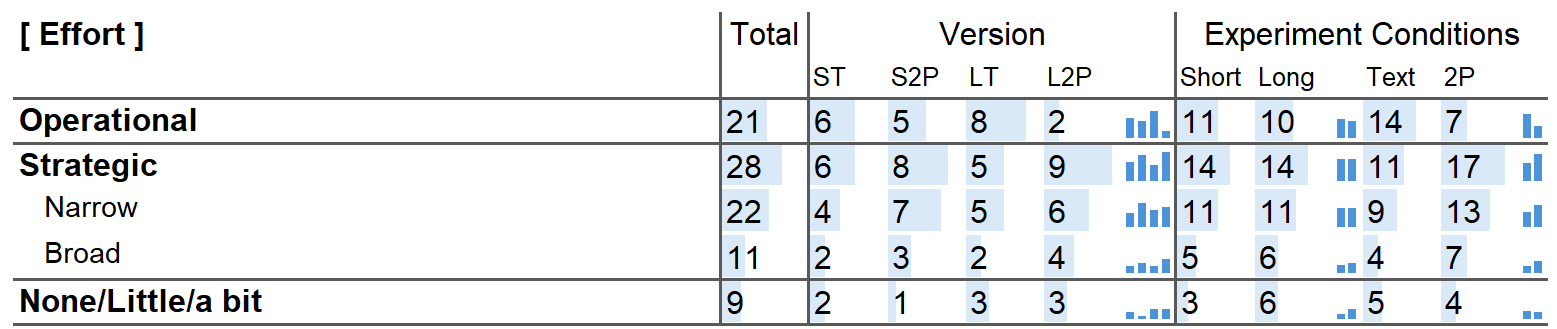
\includegraphics[width=\linewidth]{content/image/cog/effort_table.png}
\end{table}

\subsection{Source of Effort}
\label{sec:effort}

\vspace{5pt}
\begin{tldrbox}
    \faInfoCircle~\xspace\textbf{Takeaway:} Participants' effort demands stem from \textit{Operational Tasks} and \textit{Strategic Planning}. Operational tasks include navigating interfaces and managing budgets, with text interface users reporting more effort in these areas. Strategic planning involves both personal and global considerations, with interactive interface users focusing more on broader, communal values. Overall, participants using the interactive interface reported more effort from strategic planning, while those using the text interface reported more effort from operational tasks.
\end{tldrbox}
Effort refers to the amount of work required to achieve a level of performance. It includes the intensity of both mental and physical resources expended during the task.

Similar to our analysis for mental demand, we code the source of effort into to major categories:~\textit{Operational Tasks} and~\textit{Strategic Planning}.

\subsubsection{Operational Tasks} Similiar to performance, we focus on operational tasks that contributed to effort with a narrow focus including: navigating the interface, managing the budget at an operational scale (i.e., making sure not to run out of budget, making specific updates between two options), or translating an opinion to a quantifiable adjustment on the survey. These narrower low level operations involves taking effort to making updates or actions related to the interface itself. We show two examples associated with different aspects of operational tasks that influence precieved effort:

\begin{displayquote}
And then I wanted to bump up (an option) maybe to 4 or <option> to 5 and realize I couldn't. My point (number of votes) had to like back down a little bit~\ldots So that would be effort came in of how do I want to really rearrange this to make it (the budget spending) maximize?

\noindent \hfill -- S029, short text interface
\end{displayquote}

\begin{displayquote}
So it was like it was very~\ldots I have to put a lot of effort in terms of you know~\ldots think about each dimension that if I give one credit to <option name> whether it will affect my credits on <another option name>.

\noindent \hfill -- S005, long text interface
\end{displayquote}

Notably, $14$ of the $20$ participants using the text interface expressed overwhelminly mentioned sources related to such sources, compared to less than half of the participants ($N=7$) from the interactive interface, with the lowest mention by the long interactive interface group ($N=2$). We review the other category before making interpretations.

\subsubsection{Strategic Planning} Opposite to operational tasks, strategic planning follow definitions established for mental demand which involces higher level strategies to complete the survey. We further derive two distinct types of planning:~\textit{personal} and~\textit{global}.~\textit{Personal strategic planning} refers to taking effort to translate preferences onto the survey without considering governing values or broader beliefs. For example, this participant expressed effort from retrieving past experiences to inform their decisions:

\begin{displayquote}
~\bracketellipsis having that prior experience and being able to quickly link it to a tangible thing that I've experienced in my personal life.

\noindent \hfill -- S032, short text interface
\end{displayquote}

\begin{displayquote}
And really the bulk of the effort was how to rank order these (options) and allocate the resources behind the upvotes so that I can accurately depict what I want~\ldots say, a committee to focus on and allocate actual fungible resources, too. 

\noindent \hfill -- S019, long interactive interface
\end{displayquote}

While the difference in the number of citations to personal strategic planning are less pronounced across groups, the interactive interface (N=13) still scores slightly higher counts compared to the text interface (N=9).~\textit{Global strategic planning}, on the other hand, involves participants formulating strategies to align with broader, communal values. This includes ensuring fairness, considering the impact of different options on the entire community, and evaluating the complex relationships between various options. For example:

\begin{displayquote}
I think, imagining the trying to imagine every outcome trying to to imagine what what else would be encompassed, encompassed by each category.

\noindent \hfill -- S027, short interactive interface
\end{displayquote}

\begin{displayquote}
Hey, even though I don't really like this idea. But what if they're important? They sort of kind of deserve some attention~\ldots that's why I think I have the effort here.

\noindent \hfill -- S037, long interactive interface
\end{displayquote}
    
Both examples shows considerations beyond personal experiences, considering outcomes or social values. We notice that nearly twice as many participants (N=7) in the interactive interface expressed effort from global strategic efforts compared to the text interface (N=4). Altogether, we observe more participants using the interactive interface (N=17) reported sources of strategic effort compared to those using text-based interfaces (N=11). 

\begin{wrapfigure}{r}{0.45\textwidth} % Adjust the width as needed
    \centering
    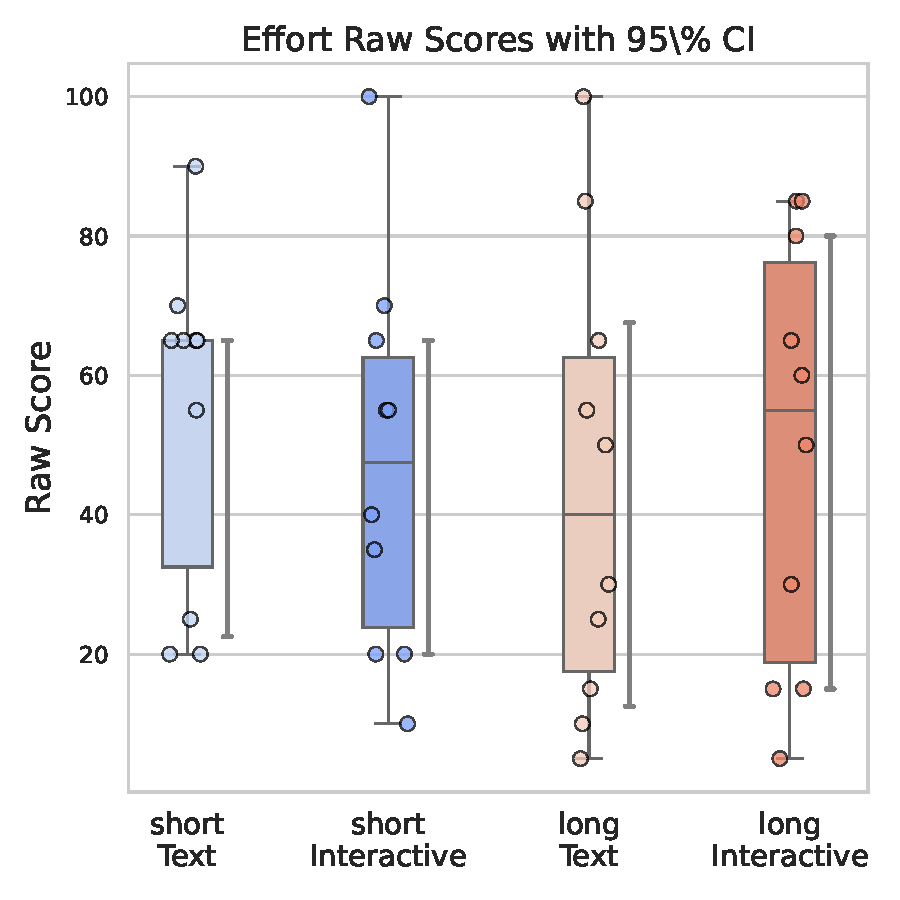
\includegraphics[width=0.45\textwidth, trim=0 13 0 13, clip]{content/image/cog/Effort_scores.pdf}
    \captionsetup{width=0.40\textwidth, justification=justified} % Adjust the width to match the image width
    \caption{Effort Raw Score: Text placed here}
    \label{fig:effort_cog_score}
\end{wrapfigure}

Qualitative analysis in this subsection added clear evidence that the source of cognitive demand for effort differs between text and interactive interfaces, similiar to mental demand. Participants using the interactive interface focus less on operational tasks and more on strategic planning, specifcially global strategic planning, where they think about options holistically and beyond the option itself. This is in contrast to participants using the text interface, who focus more on operational tasks and a narrower strategic planning scope. The raw NASA-TLX effort scores (Figure~\ref{fig:effort_cog_score}) can then be explained that even though reported values are similar across the four experiment groups, the sources of effort differ between text and interactive interfaces.

% ============================================= %
\begin{table}[h]
    \caption{Mental Demand Table, needs to be updated with some new terms definitions for some of the columns.}
    \label{tbl:fustration}
    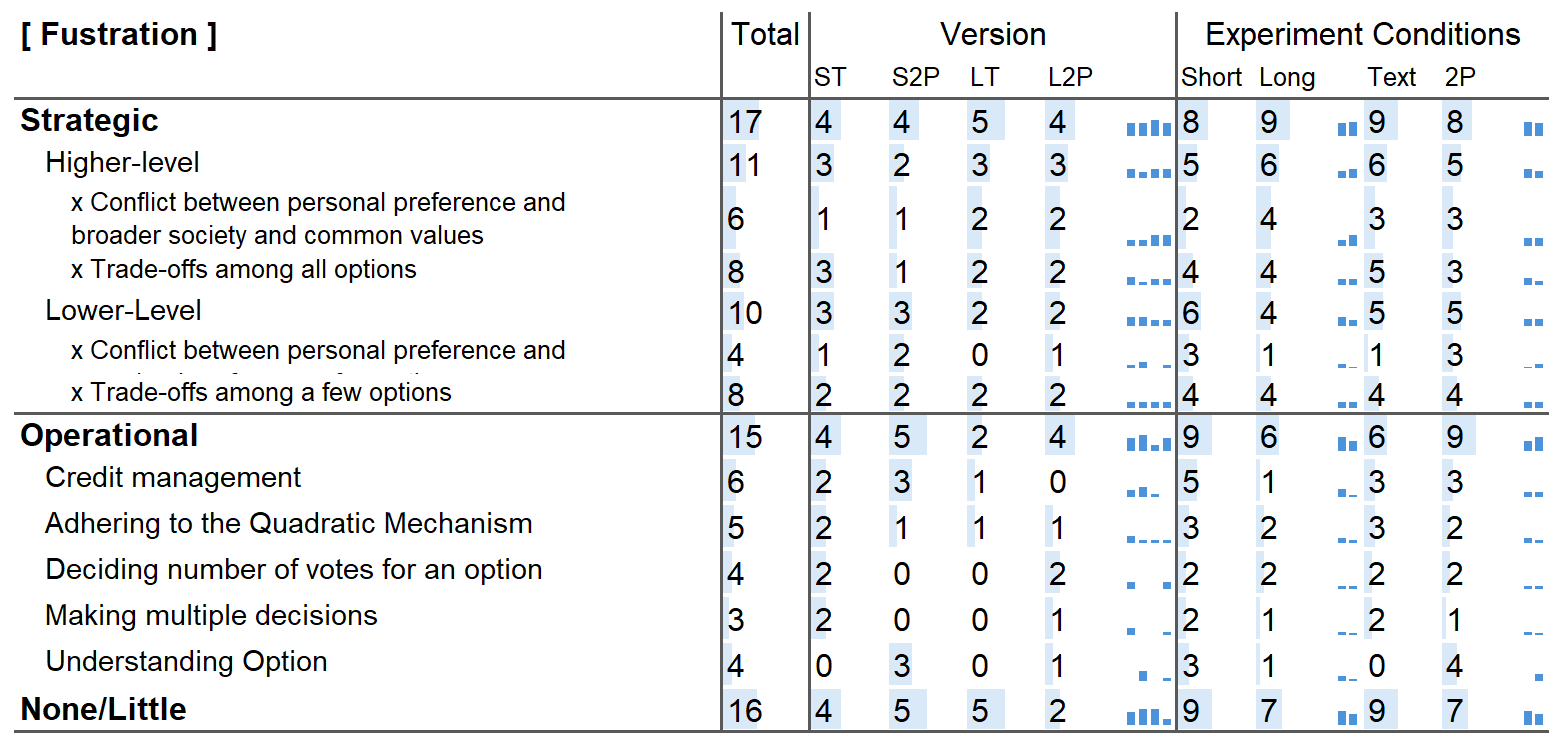
\includegraphics[width=\linewidth]{content/image/cog/fustration_table.png}
\end{table}
\subsection{Source of Physical Demand} 
\label{sec:fustration}

\vspace{5pt}
\begin{tldrbox}
    \faInfoCircle~\xspace\textbf{Takeaway:} Participants experienced frustration from two main sources: \textit{Operational Actions} and \textit{Strategic Planning}. Operational actions included managing budgets, deciding final values for options, and understanding content, with text interface users reporting more frustration in these areas. Strategic planning frustration stemmed from conflicts between personal and societal preferences and making trade-offs among options. Overall, while operational frustrations were common across all groups, participants in the long text interface reported slightly less frustration, likely due to fewer operational challenges.
\end{tldrbox}

Fustration is the last dimension of NASA-TLX. It refers to the extent to which the participant is annoyed, irritated, or discouraged during the task.

Following the previous analysis, we categorize the sources of frustration into three major themes:~\textit{Operational Actions} and~\textit{Strategic Planning}

\subsubsection{Operational Actions} Similar to the previous definitions, $15$ participants highlighted this source for frustration. Six participants expressed frustration regarding credit management (i.e., overspending budget); four participants mentioned had trouble deciding the final value for the options; three participants are frustrated because they need to make multiple decisions; five participants were frustrated with the quadratic mechanism; four participants are frustrated trying to understand the content of the option or how the option connects to them. For example, 

\begin{displayquote}
I was slightly frustrated when doing the task, probably because there was a budget that we kind of had to stick with it.

\noindent \hfill -- S001, long text interface, quadratic mechanism
\end{displayquote}

\begin{displayquote}
i think just frustration~\bracketellipsis because when i was making like the decisions on how many upvotes I could put in each section, I was running out of credits.

\noindent \hfill -- S013, short interactive interface, budget management
\end{displayquote}

These demonstrated participants frustration because they are hindered by not being able to complete specific operational actions or constraints presented by QS. What is noteable is that all experiment groups had almost half of the participants express operational frustration compared to only two participants from the long text interface group. It is not clear why they did not encounter similiar frustration.

\subsubsection{Strategic Planning} For frustration, we further derived strategic planning into two types: ~\textit{lower-level} and~\textit{higher-level}. For the former, Four participants expressed conflict between their personal preferences and what they believe would be other people's preferences. Eight participants experienced conflict between making tradeoffs among a few options. For example:

\begin{displayquote}
Because I know that's important to other people. But it just doesn't to me.
    
\noindent \hfill -- S010, short interactive interface
\end{displayquote}

\begin{displayquote}
I would have loved to have given more to other groups~\ldots and I felt stressed like~\bracketellipsis well~\ldots it's a group that you know is still~\ldots you know~\ldots important~\bracketellipsis
\noindent \hfill -- S020, long text interface
\end{displayquote}

These quotes showed participants trying to ahere to lower-level strategies such as considering personal prefernces or making trade-offs within a smaller scope. Compare to~\textit{higher-level strategic planning}, where six participants expressed conflicts that touch on the broader society and their core values of looking at the broader scope. Eight participants felt frustrated because they were forced to make trade-offs among \textit{all} options instead of a few. For example,

\begin{displayquote}
I had to consider how I feel towards that~\ldots how religious media broadcasting is being used in like today's society~\ldots today's political environment. So yeah~\ldots you really have to consider what is important to you. 
\noindent \hfill -- S020, long text interface, value conflicts
\end{displayquote}

\begin{displayquote}
I think the frustration is~\ldots I wish that we could help all of these causes, but you know it's just like anything else. You can't do everything and when it's not~\ldots  I feel like it's hard to quantify how much some of these things should be supported versus others. So when you're talking about upvotes and things that's challenging to me, it's frustrating.
\noindent \hfill -- S026, long interactive interface, considering all options
\end{displayquote}

\begin{wrapfigure}{r}{0.45\textwidth} % Adjust the width as needed
    \centering
    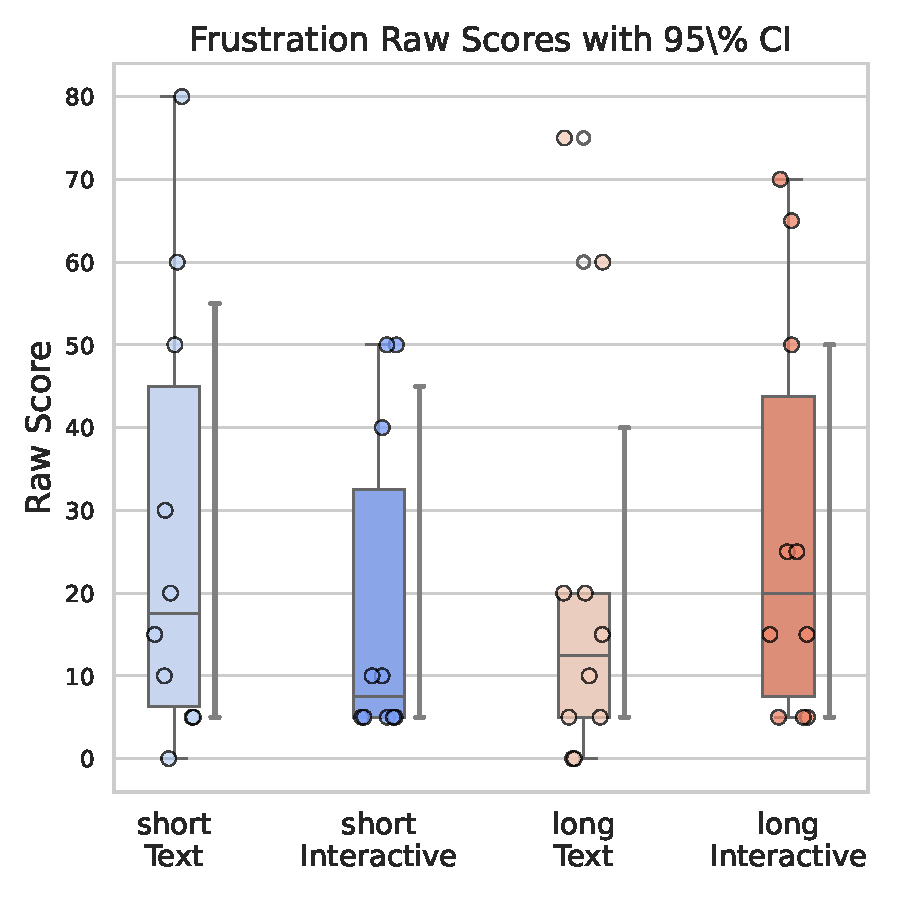
\includegraphics[width=0.45\textwidth, trim=0 13 0 13, clip]{content/image/cog/Frustration_scores.pdf}
    \captionsetup{width=0.40\textwidth, justification=justified} % Adjust the width to match the image width
    \caption{Fustration Raw Score: Participants other than the long interactive interface reported minimal physical demand. The long interactive interface had the highest physical demand, likely due to increased mouse clicks and extended time spent looking at the vertical screen.}
    \label{fig:fustration_cog_score}
\end{wrapfigure}

Fustration that stemmed from strategy planning are spread across all experimental conditions. Reflecting on the raw NASA-TLX scores (Figure~\ref{fig:fustration_cog_score}), We only see a slight difference in less frustration from the long text interface participants compared with the rest of the participants, likey due to the less frustration from operational tasks. Thus, we interpret that frustration comes more from individual's ability to discern and make decisions and not necessarily tied to specific methods in the construction of preference.

\subsection{Summary}
To recap, the analysis identified the different sources of cognitive load experienced by participants. More specifically, it highlighted differences across experimental conditions. Interactive interfaces, especially long ones, drive participants to adopt a holistic view and encourage higher-level deliberation, indicated by increased mental demand and effort. Conversely, participants perceived more operational demand when completing specific tasks using the text interface. Mental demand, effort, and temporal demand highlighted the urgency participants felt to complete tasks swiftly. This distinction doesn't mean one group of participants excludes the other group's demands, but it highlights that the main source of demand shifts with different interfaces.




% \begin{figure}[ht]
%     \centering
%     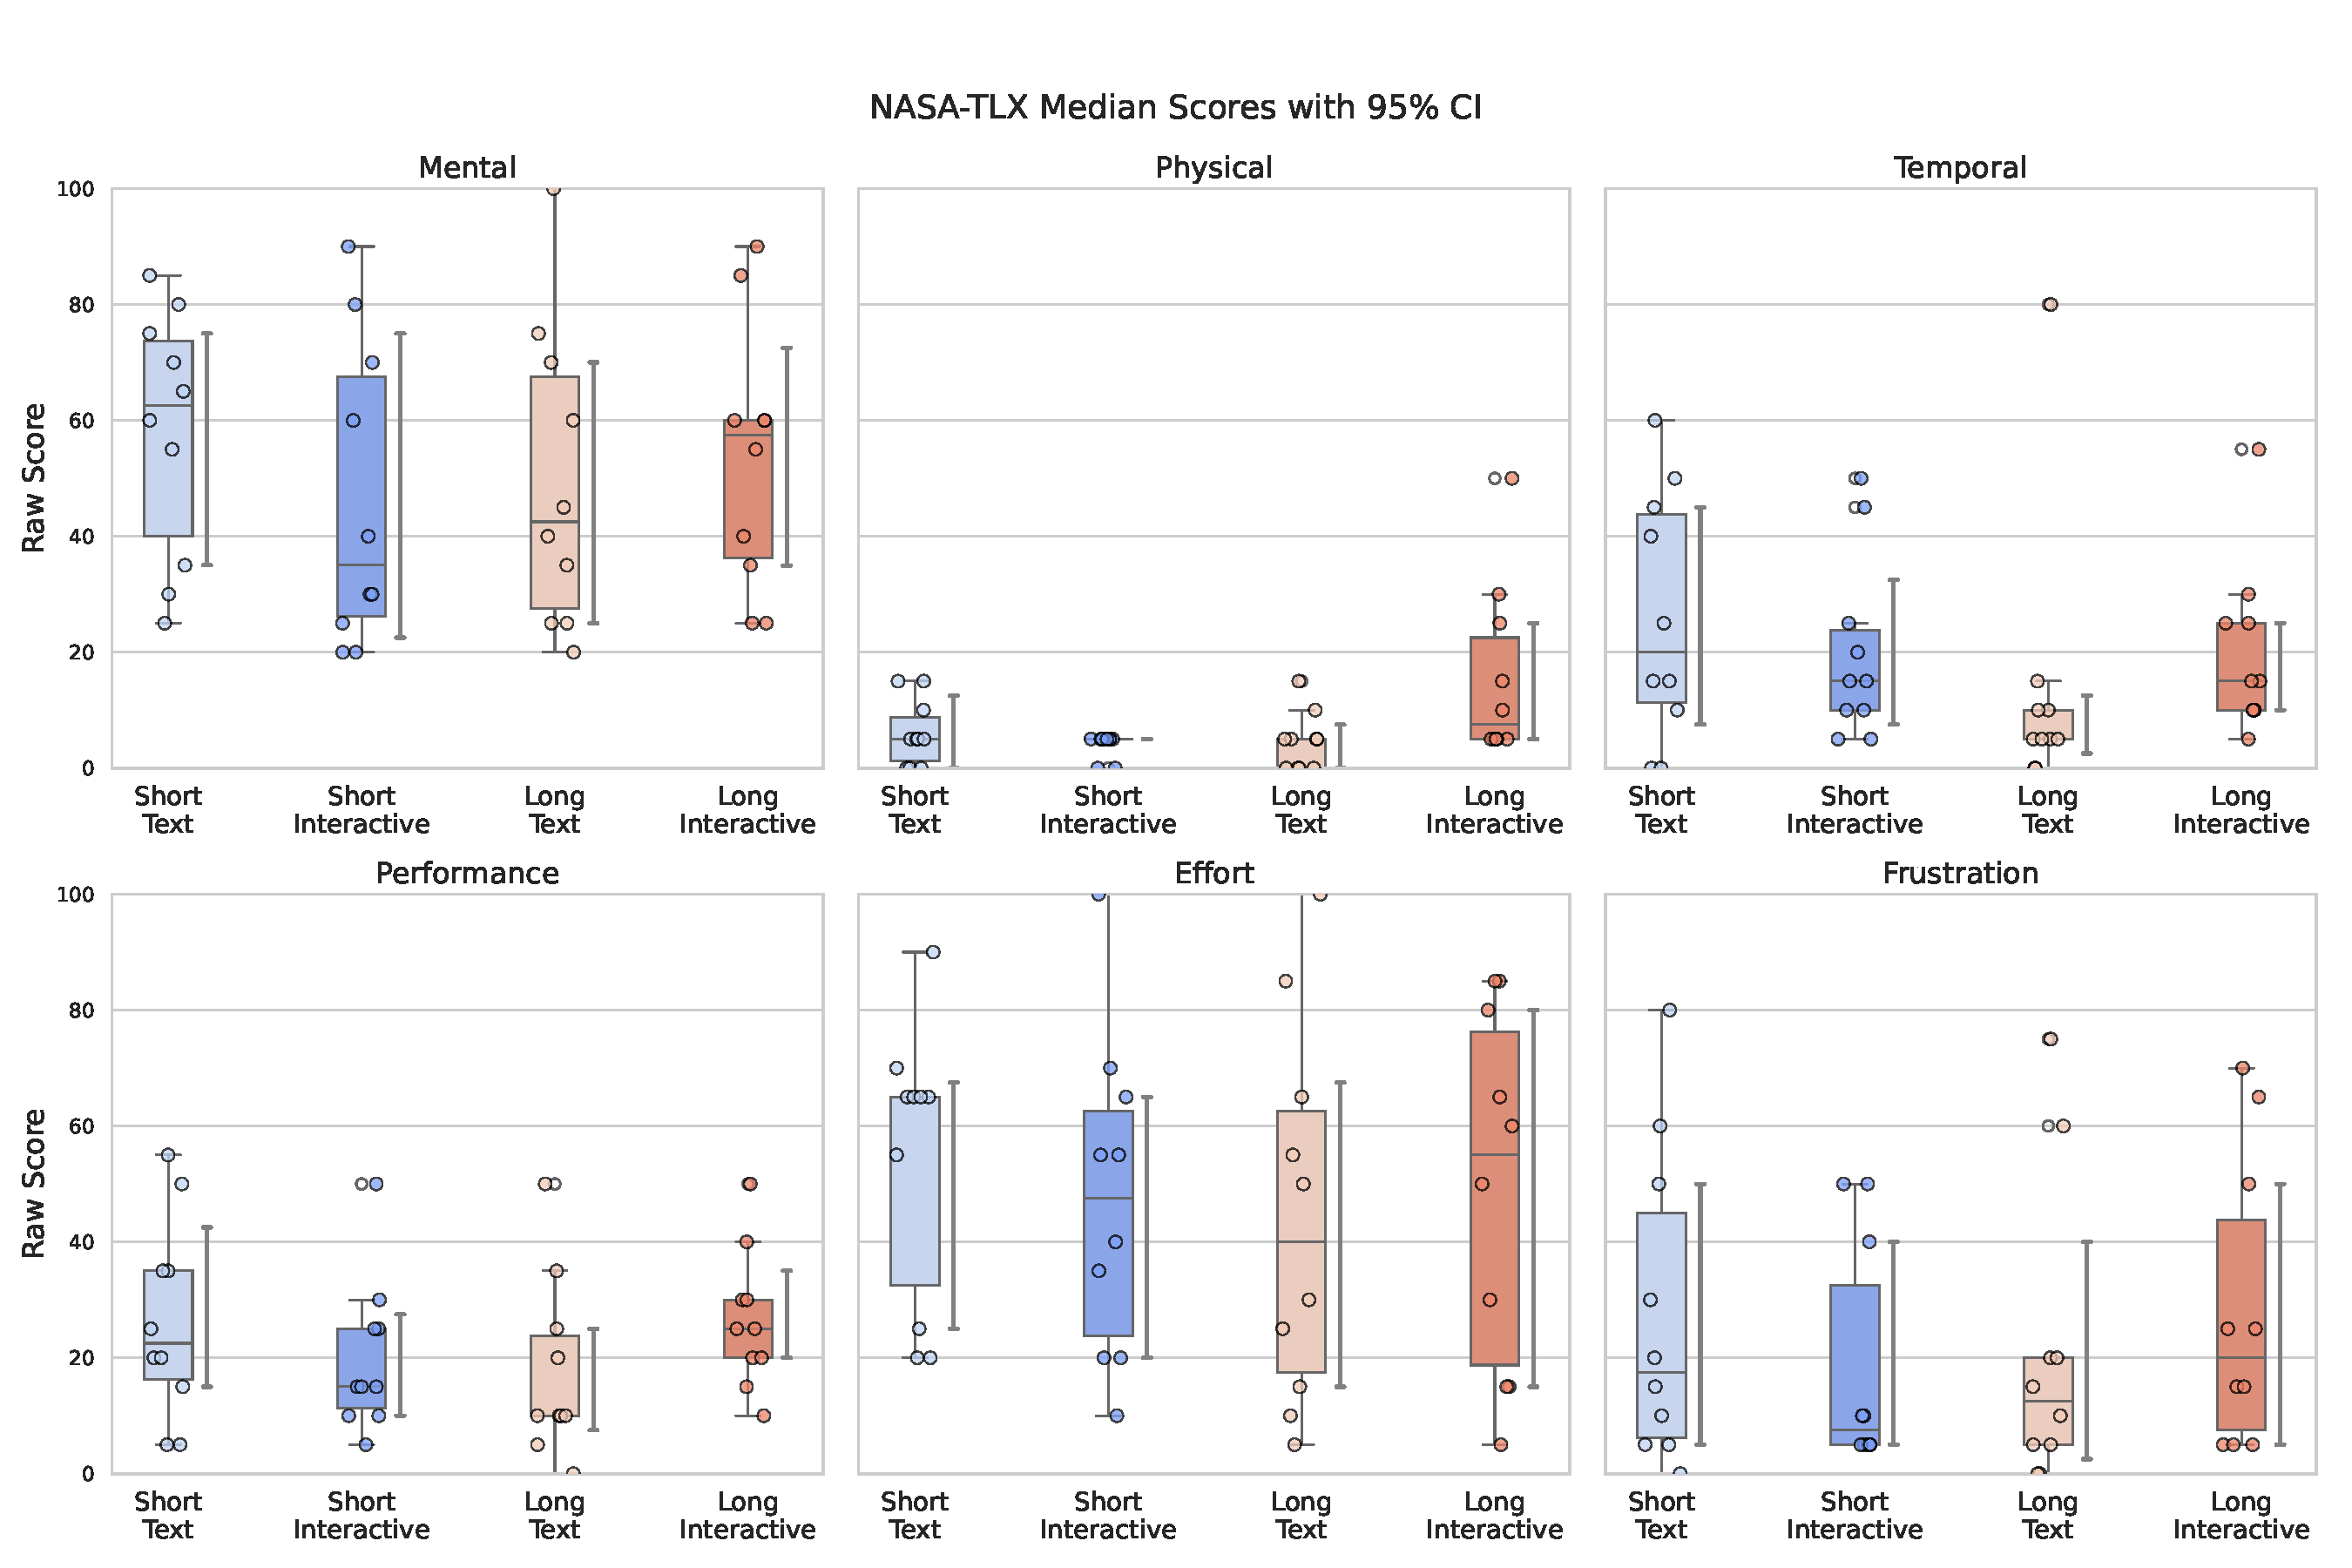
\includegraphics[width=\textwidth]{content/image/cog/nasatlx_final_value_with_CI.pdf}
%     \caption{NASA-TLX Results}
%     \label{fig:nasatlx-with-ci}
% \end{figure}